\documentclass{beamer}

% xcolor and define colors -------------------------
\usepackage{xcolor}

% https://www.viget.com/articles/color-contrast/
\definecolor{purple}{HTML}{5601A4}
\definecolor{navy}{HTML}{0D3D56}
\definecolor{ruby}{HTML}{9a2515}
\definecolor{alice}{HTML}{107895}
\definecolor{daisy}{HTML}{EBC944}
\definecolor{coral}{HTML}{F26D21}
\definecolor{kelly}{HTML}{829356}
\definecolor{cranberry}{HTML}{E64173}
\definecolor{jet}{HTML}{131516}
\definecolor{asher}{HTML}{555F61}
\definecolor{slate}{HTML}{314F4F}

% Mixtape Sessions
\definecolor{picton-blue}{HTML}{00b7ff}
\definecolor{violet-red}{HTML}{ff3881}
\definecolor{sun}{HTML}{ffaf18}
\definecolor{electric-violet}{HTML}{871EFF}

% Main theme colors
\definecolor{accent}{HTML}{00b7ff}
\definecolor{accent2}{HTML}{871EFF}
\definecolor{gray100}{HTML}{f3f4f6}
\definecolor{gray800}{HTML}{1F292D}


% Beamer Options -------------------------------------

% Background
\setbeamercolor{background canvas}{bg = white}

% Change text margins
\setbeamersize{text margin left = 15pt, text margin right = 15pt} 

% \alert
\setbeamercolor{alerted text}{fg = accent2}

% Frame title
\setbeamercolor{frametitle}{bg = white, fg = jet}
\setbeamercolor{framesubtitle}{bg = white, fg = accent}
\setbeamerfont{framesubtitle}{size = \small, shape = \itshape}

% Block
\setbeamercolor{block title}{fg = white, bg = accent2}
\setbeamercolor{block body}{fg = gray800, bg = gray100}

% Title page
\setbeamercolor{title}{fg = gray800}
\setbeamercolor{subtitle}{fg = accent}

%% Custom \maketitle and \titlepage
\setbeamertemplate{title page}
{
    %\begin{centering}
        \vspace{20mm}
        {\Large \usebeamerfont{title}\usebeamercolor[fg]{title}\inserttitle}\\
        {\large \itshape \usebeamerfont{subtitle}\usebeamercolor[fg]{subtitle}\insertsubtitle}\\ \vspace{10mm}
        {\insertauthor}\\
        {\color{asher}\small{\insertdate}}\\
    %\end{centering}
}

% Table of Contents
\setbeamercolor{section in toc}{fg = accent!70!jet}
\setbeamercolor{subsection in toc}{fg = jet}

% Button 
\setbeamercolor{button}{bg = accent}

% Remove navigation symbols
\setbeamertemplate{navigation symbols}{}

% Table and Figure captions
\setbeamercolor{caption}{fg=jet!70!white}
\setbeamercolor{caption name}{fg=jet}
\setbeamerfont{caption name}{shape = \itshape}

% Bullet points

%% Fix left-margins
\settowidth{\leftmargini}{\usebeamertemplate{itemize item}}
\addtolength{\leftmargini}{\labelsep}

%% enumerate item color
\setbeamercolor{enumerate item}{fg = accent}
\setbeamerfont{enumerate item}{size = \small}
\setbeamertemplate{enumerate item}{\insertenumlabel.}

%% itemize
\setbeamercolor{itemize item}{fg = accent!70!white}
\setbeamerfont{itemize item}{size = \small}
\setbeamertemplate{itemize item}[circle]

%% right arrow for subitems
\setbeamercolor{itemize subitem}{fg = accent!60!white}
\setbeamerfont{itemize subitem}{size = \small}
\setbeamertemplate{itemize subitem}{$\rightarrow$}

\setbeamertemplate{itemize subsubitem}[square]
\setbeamercolor{itemize subsubitem}{fg = jet}
\setbeamerfont{itemize subsubitem}{size = \small}







% Links ----------------------------------------------

\usepackage{hyperref}
\hypersetup{
  colorlinks = true,
  linkcolor = accent2,
  filecolor = accent2,
  urlcolor = accent2,
  citecolor = accent2,
}


% Line spacing --------------------------------------
\usepackage{setspace}
\setstretch{1.2}


% \begin{columns} -----------------------------------
\usepackage{multicol}


% Fonts ---------------------------------------------
% Beamer Option to use custom fonts
\usefonttheme{professionalfonts}

% \usepackage[utopia, smallerops, varg]{newtxmath}
% \usepackage{utopia}
\usepackage[sfdefault,light]{roboto}

% Small adjustments to text kerning
\usepackage{microtype}



% Remove annoying over-full box warnings -----------
\vfuzz2pt 
\hfuzz2pt


% Table of Contents with Sections
\setbeamerfont{myTOC}{series=\bfseries, size=\Large}
\AtBeginSection[]{
        \frame{
            \frametitle{Roadmap}
            \tableofcontents[current]   
        }
    }


% Tables -------------------------------------------
% Tables too big
% \begin{adjustbox}{width = 1.2\textwidth, center}
\usepackage{adjustbox}
\usepackage{array}
\usepackage{threeparttable, booktabs, adjustbox}
    
% Fix \input with tables
% \input fails when \\ is at end of external .tex file
\makeatletter
\let\input\@@input
\makeatother

% Tables too narrow
% \begin{tabularx}{\linewidth}{cols}
% col-types: X - center, L - left, R -right
% Relative scale: >{\hsize=.8\hsize}X/L/R
\usepackage{tabularx}
\newcolumntype{L}{>{\raggedright\arraybackslash}X}
\newcolumntype{R}{>{\raggedleft\arraybackslash}X}
\newcolumntype{C}{>{\centering\arraybackslash}X}

% Figures

% \imageframe{img_name} -----------------------------
% from https://github.com/mattjetwell/cousteau
\newcommand{\imageframe}[1]{%
    \begin{frame}[plain]
        \begin{tikzpicture}[remember picture, overlay]
            \node[at = (current page.center), xshift = 0cm] (cover) {%
                \includegraphics[keepaspectratio, width=\paperwidth, height=\paperheight]{#1}
            };
        \end{tikzpicture}
    \end{frame}%
}

% subfigures
\usepackage{subfigure}


% Highlight slide -----------------------------------
% \begin{transitionframe} Text \end{transitionframe}
% from paulgp's beamer tips
\newenvironment{transitionframe}{
    \setbeamercolor{background canvas}{bg=accent!40!black}
    \begin{frame}\color{accent!10!white}\LARGE\centering
}{
    \end{frame}
}


% Table Highlighting --------------------------------
% Create top-left and bottom-right markets in tabular cells with a unique matching id and these commands will outline those cells
\usepackage[beamer,customcolors]{hf-tikz}
\usetikzlibrary{calc}
\usetikzlibrary{fit,shapes.misc}

% To set the hypothesis highlighting boxes red.
\newcommand\marktopleft[1]{%
    \tikz[overlay,remember picture] 
        \node (marker-#1-a) at (0,1.5ex) {};%
}
\newcommand\markbottomright[1]{%
    \tikz[overlay,remember picture] 
        \node (marker-#1-b) at (0,0) {};%
    \tikz[accent!80!jet, ultra thick, overlay, remember picture, inner sep=4pt]
        \node[draw, rectangle, fit=(marker-#1-a.center) (marker-#1-b.center)] {};%
}

\usepackage{breqn} % Breaks lines

\usepackage{amsmath}
\usepackage{mathtools}

\usepackage{pdfpages} % \includepdf

\usepackage{listings} % R code
\usepackage{verbatim} % verbatim

% Video stuff
\usepackage{media9}

% packages for bibs and cites
\usepackage{natbib}
\usepackage{har2nat}
\newcommand{\possessivecite}[1]{\citeauthor{#1}'s \citeyearpar{#1}}
\usepackage{breakcites}
\usepackage{alltt}

% tikz
\usepackage{tikz}
\usepackage{pgfplots}
\usetikzlibrary{calc, positioning, decorations.pathreplacing, arrows.meta, intersections}
\pgfdeclarelayer{bg}
\pgfdeclarelayer{back}
\pgfdeclarelayer{fg}
\pgfsetlayers{bg,main,fg,back}
\usetikzlibrary{shapes,arrows}

% Setup math operators
\DeclareMathOperator{\E}{E} \DeclareMathOperator{\tr}{tr} \DeclareMathOperator{\se}{se} \DeclareMathOperator{\I}{I} \DeclareMathOperator{\sign}{sign} \DeclareMathOperator{\supp}{supp} \DeclareMathOperator{\plim}{plim}
\DeclareMathOperator*{\dlim}{\mathnormal{d}\mkern2mu-lim}
\newcommand\independent{\protect\mathpalette{\protect\independenT}{\perp}}
   \def\independenT#1#2{\mathrel{\rlap{$#1#2$}\mkern2mu{#1#2}}}
\newcommand*\colvec[1]{\begin{pmatrix}#1\end{pmatrix}}

\newcommand{\myurlshort}[2]{\href{#1}{\textcolor{gray}{\textsf{#2}}}}


\begin{document}

\imageframe{./lecture_includes/mixtape_ci_cover.png}


% ---- Content ----

\section{Matching and weighting}


\subsection{What is matching?}

\begin{frame}{Parameters of interest}

\begin{itemize}
	\item RCTs can recover the ATE
	\item DD and synth can identify the ATT
	\item Local average treatment effect can be identified using RDD and IV
	\item Can anything else recover the ATE and if so under what conditions?
\end{itemize}

\end{frame}



\begin{frame}{Defined causal parameters}

Recall our definition of the ATE in terms of population mean differences in potential outcomes: $$E[Y^1] - E[Y^0]$$

We work with samples, so we express the ATE sample analog: $$\frac{1}{N} \sum_i \bigg [ Y_i^1 - Y_i^0 \bigg ]$$


\end{frame}

\begin{frame}{Defined causal parameters}

Our ATE estimator is a weighted average of the ATT and the ATU:

$$\widehat{\delta}^{ATE} = \frac{N_T}{N}\  \widehat{\delta}^{ATT} + \frac{N_C}{N}\  \widehat{\delta}^{ATU}$$


where $\widehat{\delta}^{ATT} = \frac{1}{N_T} \sum_i \bigg [Y_i^1 - \widehat{Y}_i^0 \bigg ]$;
$\widehat{\delta}^{ATU} = \frac{1}{N_C} \sum_i \bigg [\widehat{Y}_i^1 - Y_i^0 \bigg ]$.


\pause\bigskip~\bigskip
What is $\widehat{Y}^0_i$ for the treatment group?  It's an \textbf{estimate} of the \textbf{missing} counterfactual.  And this is its estimated value: 
$$\widehat{Y}^0_i \equiv \frac{1}{Pr(D)} \sum_{j \in \{D_j=0\}}w_{ij}Y_j^0$$

\begin{itemize}
  \item $w_{ij}$ is the weight unit $j$ receives in predicting unit $i$'s counterfactual
\end{itemize}

\end{frame}

\begin{frame}{Estimating missing counterfactuals}

$$\widehat{Y}^0_i \equiv \frac{1}{Pr(D)} \sum_{j \in \{D_j=0\}}w_{ij}Y_j^0$$

\bigskip
We will be estimating counterfactuals as \textbf{weighted} averages over outcomes from the other group (e.g., control) by incorporating observable covariates

\begin{itemize}
  \item Matching and weighting methods will correct for relevant differences in observables, not just to do it, but because it closes the backdoor paths necessary for conditional independence to hold
  \item Estimators differ in how the weights, $w_{ij}$, are calculated
  \item Large part of the goal becomes \textbf{balance} on the conditioning set of covariates between treatment and control group needed to satisfy the backdoor criterion
\end{itemize}

\end{frame}

\subsection{Simple weighting}

\begin{frame}{Big picture}

\begin{itemize}
\item We are going to use weighting and matching methods to adjust for observable differences between treatment and control groups
\item Personal philosophy: this \textbf{must be driven} by model like reasoning as this only has any hope if the backdoor criterion holds
\item Personal observation: given the lack of comfort people have with modeling in general, it's not a good sign when you see them then use matching methods
\item Let's define the terms first: what is a covariate?
\end{itemize}

\end{frame}


\begin{frame}{Observable Covariate}
	
	
	\begin{block}{Definition: Predetermined Covariates}
	Variable $X$ is a predetermined covariate if for each individual $i$, the value of $X_i$ does not depend on treatment status.
	\end{block}
	
	\begin{itemize}
	\item Does not imply $X$ and treatment status are independent 
	\item Sometimes covariates do not change over time, but doesn't have to be 
	\item Colliders are not covariates; anything the treatment can change is not a covariate (``bad controls'', Angrist and Pischke MHE)
	\end{itemize}
	
\end{frame}

\begin{frame}{Adjustment for Observables}
	
	\begin{itemize}
	\item Simple weighting methods (e.g., subclassification)
	\item Exact matching methods (e.g., nearest neighbors)
	\item Approximate matching methods (e.g., propensity scores)
	\item Hybrid matching methods (e.g., coarsened exact matching)
	\end{itemize}


\end{frame}

\begin{frame}{History of non-experimental matching}

\begin{itemize}

	\item A set of techniques for estimating ATE emerged in the 20th century from statistics and epidemiology, largely driven by public health concerns about smoking's connection to lung cancer
	\item ``Weighting'' methods to correct for covariate imbalance were developed to estimate ATE from non-experimental data
	\item In time these evolved into matching, and while conceptually they seem distinct, they are very similar
	\item Huge area, and it never really took off in economics despite some initial promise (Dehejia and Wahba 1999; 2002), but if you take Causal Inference Part 2, you'll see that the principles are there in difference-in-differences and synthetic control


\end{itemize}

\end{frame}


\begin{frame}{Smoking thought experiment}

	\begin{center}	
    \textbf{Does Smoking Cause Cancer?}
  \end{center}

\bigskip
\begin{itemize}
	\item Split a large enough population to gain enough power to detect causal effects into treatment and control
	\item Treatment spends their lives smoking a pack of day; control abstains
	\item Compare lung cancer rates between the two groups
	\item Low realism: can't really expect people to comply with a longterm experiment like this
	\item But important, so how did scientists proceed? Through weighting-based methods
\end{itemize}

\end{frame}

\begin{frame}[plain, shrink=20]
	\begin{figure}
	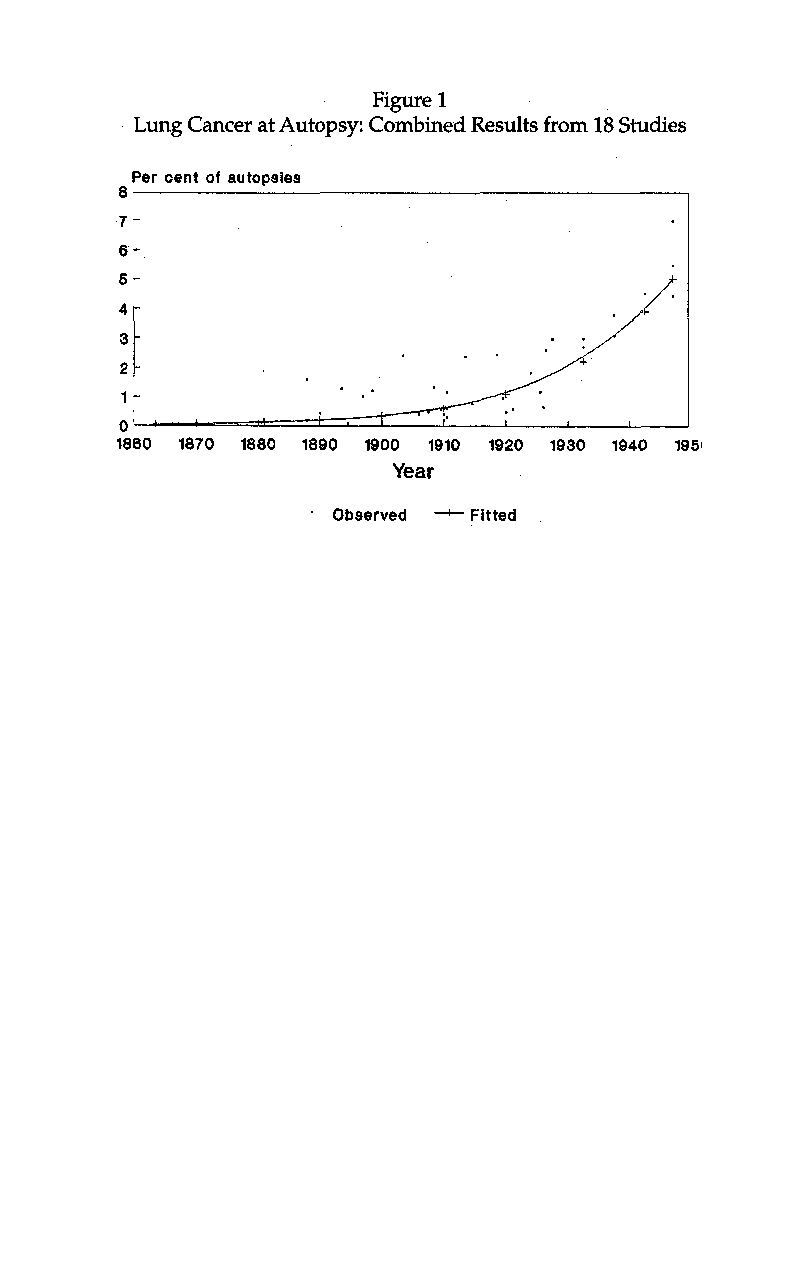
\includegraphics[scale=0.75]{./lecture_includes/cancer_fig1.pdf}
	\end{figure}

	\begin{figure}
	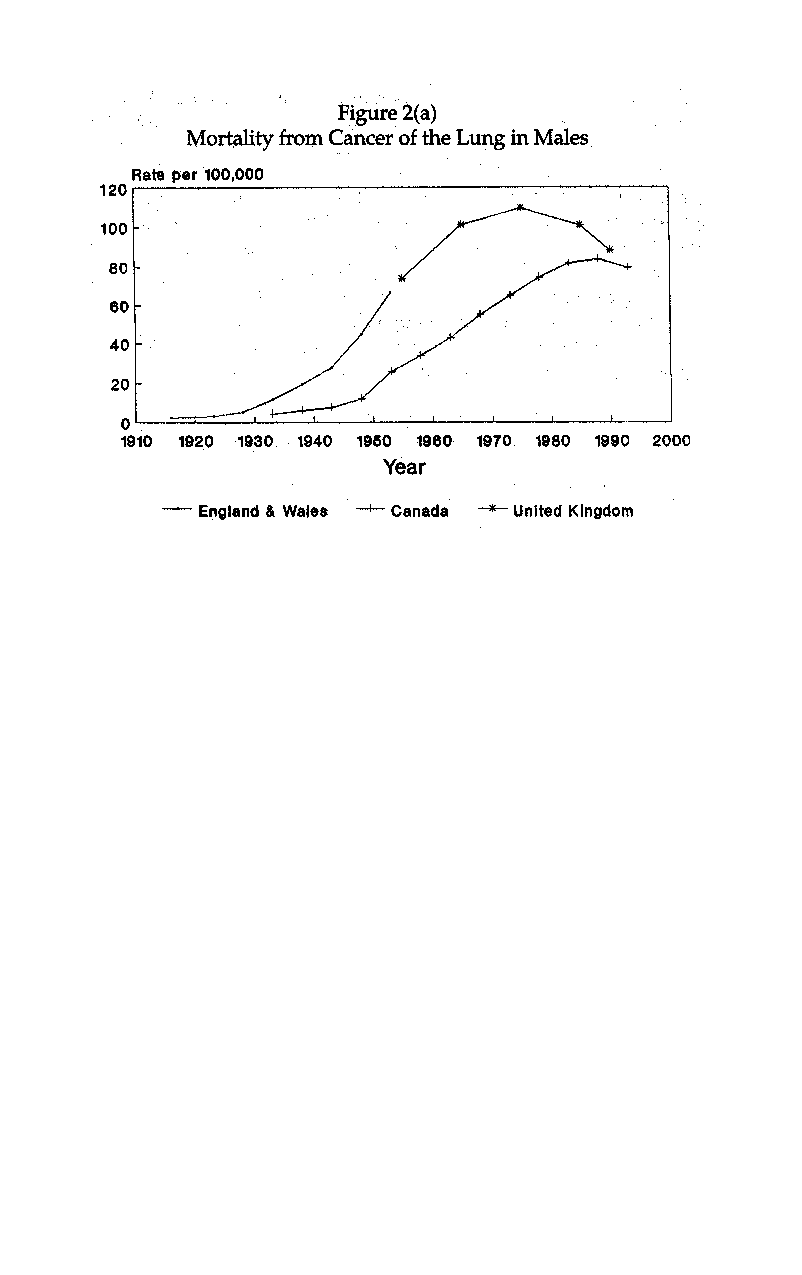
\includegraphics[scale=0.75]{./lecture_includes/cancer_fig2.pdf}
	\end{figure}

\end{frame}	


\begin{frame}[plain]
	
	\begin{figure}
	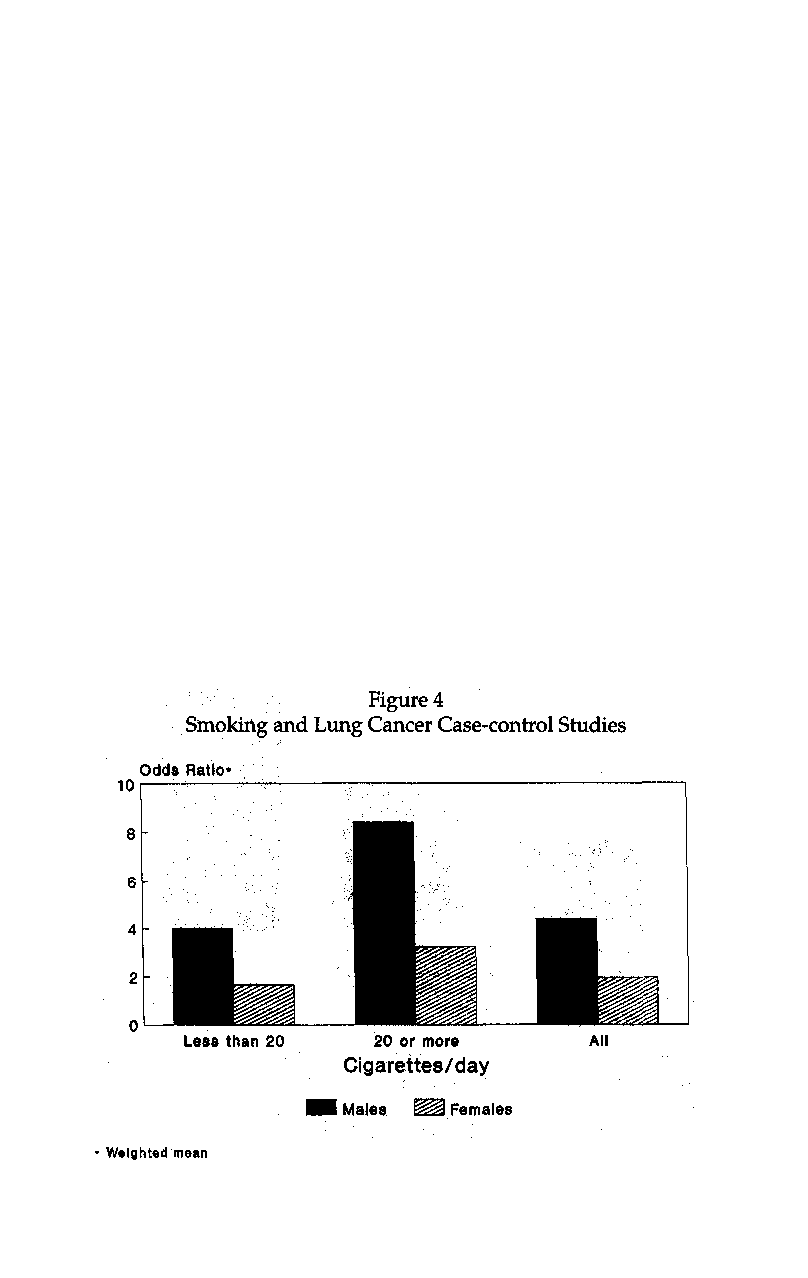
\includegraphics[scale=0.5]{./lecture_includes/smoking_figure1.pdf}
	\end{figure}

	\begin{figure}
	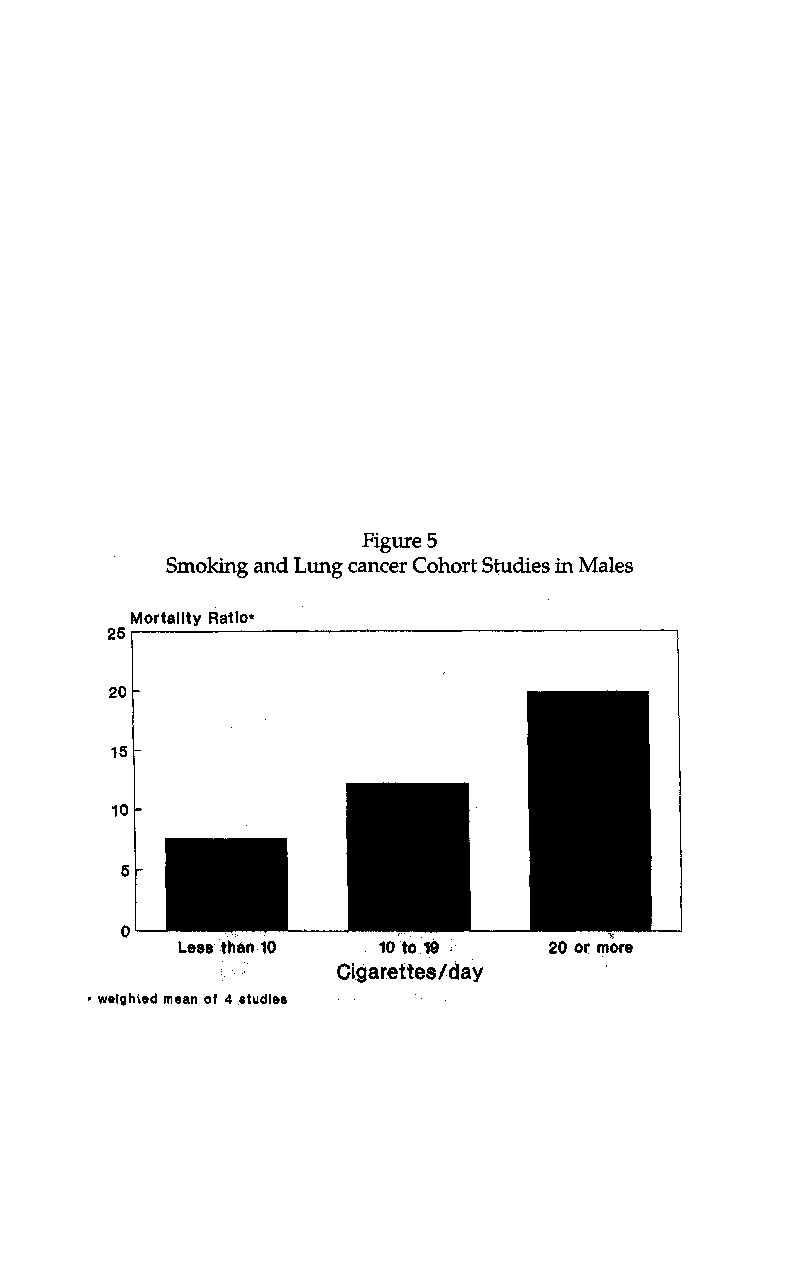
\includegraphics[scale=0.5]{./lecture_includes/smoking_figure2.pdf}
	\end{figure}

\end{frame}	
	

	
\begin{frame}{Does Smoking Cause Cancer?}
	
  Smoking, $S$, \emph{causes} lung cancer, $C$ ($S \rightarrow C$) versus spurious correlation due to the $Z$ confounder:

  \begin{center}
    \begin{tikzpicture}
    [node distance=1.5cm]

    % nodes %
    \node[text centered] (z) {$Z$};
    \node[below right of = z, text centered] (c) {$C$};
    \node[below left of = z, text centered] (s) {$S$};
    
    % edges %
    \draw[->, line width= 0.5] (z) -- (c);
    \draw[->, line width= 0.5] (z) -- (s);
    % \draw[->, line width= 0.5] (s) -- (c);
    
    \end{tikzpicture}
  \end{center}

Legitimate criticism at the time, but incorrect in hindsight -- hindsight is 20/20
	
\end{frame}


\begin{frame}{Nature of the criticism}

Other criticisms came from giants like Joseph Berkson, Jerzy Neyman and Ronald Fisher
		\begin{enumerate}
		\item Correlation b/w smoking and lung cancer was spurious due to biased selection of subjects
		\item Complaints about functional forms using ``risk ratios'' and ``odds ratios''
		\item Implausible magnitudes
		\item Killer critique: \emph{no experimental evidence} to incriminate smoking as a cause of lung cancer
		\end{enumerate}
\end{frame}

\begin{frame}{Fisher's confounding theory}
		\begin{itemize}
		\item  Fisher was a chain smoking pipe smoker, he died of cancer, and he was a paid expert witness for the tobacco industry
		\item He was also equally famous as a geneticist and arguing from logic, statistics and genetic evidence proposed a hypothetical confounding genome, $Z$, which introduced selection bias into contrasts of smokers and non-smokers (``perfect doctor'')
		\item There was support for this:  studies showed that cigarette smokers and non-smokers were different on observables -- more extraverted than non-smokers and pipe smokers, differed in age, differed in income, differed in education, etc.
		\end{itemize}
\end{frame}

\begin{frame}{Broken clocks are sometimes right}
	
  \begin{itemize}
		\item Always easy to criticize someone when we look back with more information 
		\item Evidence for the \emph{causal} link was shallow: 
  \end{itemize}

  \begin{quote}  
    ``the [epidemiologists] turned out to be right, but only because bad logic does not necessarily lead to wrong conclusions.'' Robert Hooke (1983)
  \end{quote}
	
  \begin{itemize}
    \item Scientists shifted to fixing their broken clocks for good
  \end{itemize}

\end{frame}


\begin{frame}{Observable selection bias}
	
	\begin{table}\centering
		\caption{Death rates per 1,000 person-years (Cochran 1968)}
		\begin{center}
		\begin{tabular}{lccc}
		\hline \hline
		\multicolumn{1}{l}{Smoking group}&
		\multicolumn{1}{c}{Canada}&
		\multicolumn{1}{c}{U.K.}&
		\multicolumn{1}{c}{U.S.}\\
		\hline
		Non-smokers & 20.2 & 11.3 & 13.5\\
		Cigarettes & 20.5 & 14.1 & 13.5 \\
		Cigars/pipes & 35.5 & 20.7 & 17.4\\
		\hline
		\end{tabular}
		\end{center}
	\end{table}
	
Cigars in these data had much higher mortality rates in all three countries than non-smokers, but even cigarette smokers.  Cigarette smokers in Canada have same mortality rates as non-smokers. Strange associations to us today, so imagine back then when the smoking-cancer hypothesis was not settled
	
\end{frame}

\begin{frame}{Non-smokers and smokers differ in age}
	


	\begin{table}\centering
		\caption{Mean ages, years (Cochran 1968)}
		\begin{center}
		\begin{tabular}{lccc}
		\hline \hline
		\multicolumn{1}{l}{Smoking group}&
		\multicolumn{1}{c}{Canada}&
		\multicolumn{1}{c}{U.K.}&
		\multicolumn{1}{c}{U.S.}\\
		\hline
		Non-smokers & 54.9 & 49.1 & 57.0\\
		Cigarettes & 50.5 & 49.8 & 53.2 \\
		Cigars/pipes & 65.9 & 55.7 & 59.7\\
		\hline
		\end{tabular}
		\end{center}
	\end{table}
	
	\begin{itemize}
	\item Older people die at a higher rate, but for reasons other than just smoking cigars
	\item Could cigar smokers have higher observed death rates because they're older on average?
	\item How can we check this?
	\end{itemize}
 

\end{frame}

\begin{frame}{Force groups to have the same age distribution}
	
  Covariates are \emph{not balanced} -- their mean values differ for treatment and control group. 

  \bigskip 
  \textbf{Option 1: Strata}
  \begin{itemize}
    \item Compare mortality rates across the different smoking groups but \emph{within} each age group 
    \item Compare within covariate strata and then combine differences to neutralize observed confounders
  \end{itemize}

  \bigskip 
  \textbf{Option 2: Weights}
  \begin{itemize}
    \item Weight the data so that covariates are balanced, then compare mortality across treatment and control
    \item Which weights?
	\end{itemize}
\end{frame}

\begin{frame}{Weighting the data}

  Divide the smoking group samples into age groups:
  \begin{enumerate}
		\item Calculate mortality rates separately for each age group \emph{by treatment and control separately}
		\item Construct ``probability weights'': the proportion of each smoking group sample within a given age group
		\item For treatment and control group, compute the weighted averages of the age groups mortality rates using the probability weights
  \end{enumerate}
This interestingly will balance the observed covariate, age, between treatment and control


\end{frame}


\begin{frame}{Simple weighting example}
	


	\begin{table}\centering
		\begin{center}
		\begin{tabular}{lccc}
		\hline \hline
		\multicolumn{1}{l}{}&
		\multicolumn{1}{c}{Death rates}&
		\multicolumn{2}{c}{Number of}\\
		\multicolumn{1}{l}{}&
		\multicolumn{1}{c}{Pipe-smokers}&
		\multicolumn{1}{c}{Pipe-smokers}&
		\multicolumn{1}{c}{Non-smokers}\\
		\hline
		Age 20-50 & 15 & 11 & 29 \\
		Age 50-70 & 35 & 13 & 9 \\
		Age $+$70 & 50 & 16 & 2 \\
		Total & & 40 & 40 \\		
		\hline
		\end{tabular}
		\end{center}
	\end{table}
	
	\begin{flalign*}
    \only<1-2>{&\text{Question: What is the average death rate for pipe smokers?}&}\\
    \only<2-2>{&15\cdot\left(\frac{11}{40}\right)+35\cdot\left(\frac{13}{40}\right)+50\cdot\left(\frac{16}{40}\right)=35.5} \\
    \only<3-4>{&\text{Counterfactual question: What would the average mortality rate be for }} \\ 
    \only<3-4>{&\text{pipe smokers if they had the same age distribution as the non-smokers?}}\\
    \only<4-4>{&15\cdot\left(\frac{29}{40}\right)+35\cdot\left(\frac{9}{40}\right)+50\cdot\left(\frac{2}{40}\right)=21.2}
	\end{flalign*}

\end{frame}


\begin{frame}[plain]

	\begin{table}\centering
	\caption{Adjusted death rates using 3 age groups (Cochran 1968)}
		\begin{center}
		\begin{tabular}{lccc}
		\hline \hline
		\multicolumn{1}{l}{Smoking group}&
		\multicolumn{1}{c}{Canada}&
		\multicolumn{1}{c}{U.K.}&
		\multicolumn{1}{c}{U.S.}\\
		\hline
		Non-smokers & 20.2 & 11.3 & 13.5 \\
		Cigarettes & 28.3 & 12.8  &  17.7 \\
		Cigars/pipes & 21.2 & 12.0 & 14.2 \\
		\hline
		\end{tabular}
		\end{center}
	\end{table}

\end{frame}


\begin{frame}{Assumptions, data and statistics}

We need three things to estimate a causal effect
\begin{itemize}
\item \textbf{Assumptions}: what must we assume is true so that our models work with data?
\item \textbf{Data}: what data with what covariates and outcomes do we need for this project?
\item \textbf{Statistical models}: sometimes called ``estimators'' which are the calculators turning data into unbiased estimates of treatment effects (or not!)
\end{itemize}

\end{frame}

\begin{frame}{Assumption I: Independence}
	
	\begin{itemize}
	\item Randomized treatment assignment guarantees ``independence'' $$(Y^0,Y^1)\independent{D}$$
	\item Independence allows to estimate accurate causal effects through simple methods like differences in averages
		\begin{eqnarray*}
		E[Y|D=1] - E[Y|D=0] &=& \underbrace{E[Y^1|D=1] - E[Y^0|D=0]}_{\mathclap{\text{by the switching equation}}} \\
		&=& \underbrace{E[Y^1] - E[Y^0]}_{\mathclap{\text{by independence}}} \\
		&=& \underbrace{E[Y^1-Y^0]}_{\mathclap{\text{ATE}}}
		\end{eqnarray*}
	\end{itemize}
\end{frame}

\begin{frame}{Covariate distribution}

\begin{itemize}
\item Just like independence implies balance on potential outcomes, it also implies balance on covariates which is called ``common support''
\item We saw this in our Thornton regressions: cash vouchers were not associated with being male, one's age, etc.
\item If we have balance on potential outcomes, that's all we need but balance on covariates is often used to provide some evidence the randomization was done well
\end{itemize}
\end{frame}

\begin{frame}{Violations of independence}

\begin{itemize}
\item Problem with smoking and cancer was smoking wasn't \emph{randomly assigned} -- it was chosen by the ``perfect doctor'' (i.e., self selection into smoking based on factors related to potential outcomes)
\item When a treatment is ``dependent'' on potential outcomes, it means people smoke because they expect something is better when they smoke ($Y^1$) than when they don't ($Y^0$) introducing selection bias and potentially heterogenous treatment effect bias
\item Naive comparisons can be deeply misleading -- covariate adjustment can resolve this if ``conditional independence'' happens in the data
\end{itemize}

\end{frame}



\begin{frame}[plain]

	\begin{block}{Identifying assumption I: Conditional independence}
	$(Y_i^0$, $Y_i^1)$ $\independent{D} | X_i$. There exists a set $X$ of observable covariates such that after controlling for these covariates, treatment assignment is \emph{independent of potential outcomes}.
	\end{block}
	
	\begin{itemize}
	\item Conditional on $X$, treatment assignment is `as good as random'. 
	\item `As good as random' is English for ``independent of potential outcomes'' potential outcomes jargon
	\end{itemize}
\end{frame}

\begin{frame}[plain]

	\begin{block}{Identifying assumption II: Common support}
	For ranges of $X$, there is a positive probability of being both treated and untreated
	\end{block}
	
	\begin{itemize}
	\item Assumption requires that there are units in both treatment and control for the range of $X$
	\item Common support ensures we can find similar enough donors in the control pool
	\item We can't check for balance on potential outcomes, because of switching equation eliminating counterfactuals, but we can check for common support 
	\end{itemize}
\end{frame}




\begin{frame}{Big picture of conditional independence}

\begin{itemize}
\item You use these methods if you are confident in your DAG, \textbf{and} there exists a conditioning strategy that satisfies the backdoor criterion
\item If you literally refuse to commit to a model, theory of DGP or DAG, then you cannot justify matching
\item Matching is for experts -- not because it's hard, but because experts are often the ones who \emph{are willing} to write down a DAG; it rewards domain specific human capital 
\item But remember the audience and the progression away from models that Card (2014) mentioned \dots
\end{itemize}

\end{frame}


\begin{frame}{Independence breaks down under perfect doctor reasoning}

\begin{itemize}
\item Independence was violated if the treatment was assigned \emph{because} we expected things to improve or not (``perfect doctor'' reasoning)
\item If you take an action because you think it helps and others don't take the action because they don't or can't, then it is a violation of independence probably
\item Keep telling yourself this phrase: ``Firms don't flip coins to set prices''. They set prices based on profit maximization or cost minimization or equivalent goals
\item Selection bias then will be baked into those non-experimental observations and thus can't be relied on without causal inference adjustments
\end{itemize}

\end{frame}

\begin{frame}{Conditional independence}

\begin{itemize}
\item DAG reasoning can be a little unhelpful at times once we try to articulate the conditional independence assumption, so hear me out:
\item Firms don't flip coins to set prices, but is there \emph{some} random price setting conditional on observable factors (which only employees, managers and executives could possibly know about)? 
\item If they flip coins conditional on something, then that's ``conditional independence''. See -- it's a strong belief.  
\item Conditional independence means that once we adjust for covariates, all remaining variation in treatment assignment had nothing to do with profit maximization or potential outcomes more generally but rather was as good as random
\end{itemize}

\end{frame}

\begin{frame}{Identification under conditional independence}
	
Identification assumptions:
  \begin{enumerate}
		\item $(Y^1,Y^0) \independent{D} | X$ (conditional independence)
		\item $0<Pr(D=1|X)<1$ with probability one (common support)
  \end{enumerate}

\bigskip
Comparing two individuals \emph{who have the same values of} $X$, treatment is independent of potential outcomes. 

\bigskip

The second term implies we have people in treatment and control for every strata of $X$
\end{frame}


\begin{frame}{Implications of assumptions}


	\begin{itemize}
	\item Assumption 1 lets you plug $Y$ for $Y^j$ with the switching equation
		\begin{eqnarray*}
		E[Y^1-Y^0|X] &=& E[Y^1 - Y^0 | X,D=1] \\
		&=&E[Y|X,D=1] - E[Y|X,D=0]
		\end{eqnarray*}
	\item Assumption 2 lets you properly weight over the covariate distribution
		\begin{eqnarray*}
		\delta_{ATE} &=&E[Y^1-Y^0] = E\bigg[ E[Y^1 - Y^0 \ \vert \ X] \bigg] \\
		&=& \int E[Y^1 - Y^0 |X,D=1] dPr(X) \\
		&=& \int \left(E[Y|X,D=1] - E[Y|X,D=0]\right)dPr(X)
		\end{eqnarray*}
	\end{itemize}

\end{frame}




\begin{frame}{Can we defend any conditional independence?}

Other versions of conditional independence (and this shows up in diff-in-diff too)

\begin{enumerate}
  \item $Y^0 \independent{D} | X$ 
  \item $Pr(D=1|X)<1$ (with $Pr(D=1)>0$)
\end{enumerate}

\bigskip
Notice how there is only one potential outcome in the independence equation.  That's okay.  We can still then estimate the ATT (just not the ATE).

\end{frame}

\begin{frame}{ATT}

Conditional independence of $D$ with respect to $Y^0$ conditional on $X$, but not $Y^1$, lets us recover the ATT with weights and the realized data
		\begin{eqnarray*}
		\delta_{ATT} &=& E\bigg[ E[Y^1-Y^0 | D=1,X] \bigg] \\
		&=& \int \left(E[Y|X,D=1] - E[Y|X,D=0]\right)dPr(X|D=1)
		\end{eqnarray*}
\end{frame}


\begin{frame}{Summarizing}


Weighted averages under either assumption:
		\begin{eqnarray*}
		\delta_{ATE} &=& \int \left(E[Y|X,D=1] - E[Y|X,D=0]\right)dPr(X) \\
		\delta_{ATT} &=& \int \left(E[Y|X,D=1] - E[Y|X,D=0]\right)dPr(X|D=1)
		\end{eqnarray*}
ATE needs independence with respect to both potential outcomes; ATT only needs it with respect to $Y^0$. 		
		
\end{frame}

\begin{frame}{Weighting by Age ($K=2$)}
	
	\begin{table}\centering
		\begin{center}
		\begin{tabular}{lccccc}
		\hline \hline
		\multicolumn{1}{l}{}&
		\multicolumn{2}{c}{Death Rate}&
		\multicolumn{1}{c}{}&
		\multicolumn{2}{c}{Number of}\\

		\multicolumn{1}{l}{$X_k$}&
		\multicolumn{1}{c}{Smokers}&
		\multicolumn{1}{c}{Non-smokers}&
		\multicolumn{1}{c}{Diff.}&
		\multicolumn{1}{c}{Smokers}&
		\multicolumn{1}{c}{Non-smokers}\\
		\hline
		Old & 28 & 24 & 4 & 3 & 10 \\
		Young & 22 & 16 & 6 & 7 & 10 \\
		Total & & & & 10 & 20 \\
		\hline
		\end{tabular}
		\end{center}
	\end{table}
	
	

	\begin{flalign*}
		    \only<1-2>{&\text{Question: What is $\widehat{\delta_{ATE}}=\sum_{k=1}^K(\overline{Y}^{1,k} - \overline{Y}^{0,k})\cdot \left(\frac{N^k}{N}\right)$?}&}\\
		    \only<2-2>{&4\cdot\left(\frac{13}{30}\right)+6\cdot\left(\frac{17}{30}\right)=5.13} \\
		    \only<3-4>{&\text{Question: What is $\widehat{\delta_{ATT}}=\sum_{k=1}^K(\overline{Y}^{1,k} - \overline{Y}^{0,k})\cdot \left(\frac{N^k_T}{N_T}\right)$?}} \\ 
		    \only<4-4>{&4\cdot\left(\frac{3}{10}\right)+6\cdot\left(\frac{7}{10}\right)=5.4} 
	\end{flalign*}

\end{frame}
	
		
 

\begin{frame}[shrink=20,plain]{Weighting by Age and Gender ($K=4$)}
	
	\begin{table}\centering
		\begin{center}
		\begin{tabular}{lccccc}
		\hline \hline
		\multicolumn{1}{l}{}&
		\multicolumn{2}{c}{Death Rate}&
		\multicolumn{1}{c}{}&
		\multicolumn{2}{c}{Number of}\\

		\multicolumn{1}{l}{$X_k$}&
		\multicolumn{1}{c}{Smokers}&
		\multicolumn{1}{c}{Non-smokers}&
		\multicolumn{1}{c}{Diff.}&
		\multicolumn{1}{c}{Smokers}&
		\multicolumn{1}{c}{Non-smokers}\\
		\hline
		Old Males & 28 & 22 & 4 & 3 & 7 \\
		Old Females &   & 24 &   &   & 3 \\
		Young Males & 21 & 16 & 5 & 3 & 4 \\
		Young Females & 23 & 17 & 6 & 4 & 6 \\
		Total & & & & 10 & 20 \\
		\hline
		\end{tabular}
		\end{center}
	\end{table}
	
	

	\begin{flalign*}
		    \only<1-2>{&\text{Problem: What is $\widehat{\delta_{ATE}}=\sum_{k=1}^K(\overline{Y}^{1,k} - \overline{Y}^{0,k})\cdot \left(\frac{N^k}{N}\right)$?}&}\\
		    \only<2-2>{&\text{Not identified! What went wrong?}} \\
		    \only<3-4>{&\text{Question: What is $\widehat{\delta_{ATT}}=\sum_{k=1}^K(\overline{Y}^{1,k} - \overline{Y}^{0,k})\cdot \left(\frac{N^k_T}{N_T}\right)$?}} \\ 
		    \only<4-4>{&4\cdot\left(\frac{3}{10}\right)+5\cdot\left(\frac{3}{10}\right)+6\cdot\left(\frac{4}{10}\right)=5.1}
	\end{flalign*}

\end{frame}

\begin{frame}{Curse of Dimensionality}
	
	\begin{itemize}
	\item Simple weighting methods may become less feasible in finite samples as the number of covariates grows (e.g., $K=4$ was too many for this sample)
	\item Assume we have $k$ covariates and we divide each into 3 coarse categories (e.g., age: young, middle age, old; income: low, medium, high, etc.)
	\item The number of sub classification cells (or ``strata'') is $3^k$. For $k=10$, then it's $3^{10}=59,049$
	\end{itemize}
\end{frame}

\begin{frame}{Curse of Dimensionality}
	
	\begin{itemize}
	\item If sparseness occurs, it means many cells may contain either only treatment units or only control units but not both.  If so, we cannot use this kind of simple weighting (e.g., subclassification, stratification).
	\item Simple weighting methods is also a problem if the cells are ``too coarse''.  
	\item We can always use ``finer'' classifications, but finer cells worsens the dimensional problem, so we don't gain  much from that.  ex: using $10$ variables and $5$ categories for each, we get $5^{10} = 9,765,625$.  
	\item Matching methods really force us to see these curses; they're often hidden from OLS because OLS doesn't tell us it is just doing various extrapolations
	\end{itemize}
\end{frame}	


\subsection{Nearest neighbor matching}

\begin{frame}{To Look Like Someone Else}

\begin{itemize}
\item Not sure of the exact history of matching, but the idea is super intuitive
\item What if we could make synthetic xerox copies of ourselves in counterfactual states?
\item Matching is to basically find units in the control group, or treatment group, that ``look like me'' \textbf{on observables}
\item But remember -- it's driven by DAG reasoning; you only need to look minimally ``like'' the other person to satisfy backdoor
\end{itemize}

\end{frame}

\begin{frame}{Nearest Neighbor Matching}
	
	\begin{itemize}
	\item See Abadie and Imbens (2006). ``Large sample properties of matching
        estimators for average treatment effects''.  \emph{Econometrica}
	\item We could also estimate $\delta_{ATT}$ by \emph{imputing} the missing potential outcome of each treatment unit $i$ using the observed outcome from that outcome's ``nearest'' neighbor $j$ in the control set
		\begin{eqnarray*}
		\delta_{ATT} = \frac{1}{N_T}\sum_{D_i=1} (Y_i - Y_{j(i)})
		\end{eqnarray*}where $Y_{j(i)}$ is the observed outcome of a control unit such that $X_{j(i)}$ is the \textbf{closest} value to $X_i$ among all of the control observations (eg match on $X$)
	\end{itemize}
\end{frame}

\begin{frame}{Matching}
	
	\begin{itemize}
	\item We could also use the average observed outcome over $M$ closest matches:
		\begin{eqnarray*}
		\delta_{ATT} = \frac{1}{N_T}\sum_{D_i=1}\left(Y_i-\left[\frac{1}{M}\sum_{m=1}^MY_{j_m(1)}\right]\right)
		\end{eqnarray*}
	\item Works well when we can find good matches for each treatment group unit, so $M$ is usually defined to be small (i.e., $M=1$ or $M=2$)
	\end{itemize}
\end{frame}

\begin{frame}{Matching}
	
	\begin{itemize}
	\item We can also use matching to estimate $\delta_{ATE}$.  In that case, we match in both directions:
		\begin{enumerate}
		\item If observation $i$ is treated, we impute $Y^0_i$ using the control matches,     $\{Y_{j_1(i)}, \dots, Y_{j_M(i)}\}$
		\item If observation $i$ is control, we impute $Y^1_i$ using the treatment matches, $\{Y_{j_1(i)}, \dots, Y_{j_M(i)}\}$
		\end{enumerate}
	\item The estimator is:$$\widehat{\delta}_{ATE} = \frac{1}{N} \sum_{i=1}^N (2D_i -1) \left[ Y_i - \left( \frac{1}{M} \sum_{m=1}^M Y_{j_m(i)} \right) \right]$$	
	\end{itemize}
	
\end{frame}


\begin{frame}{Matching example with single covariate}
	
	\begin{table}
	\begin{tabular}{c|c|c|c|c}
	\hline
	$i$ & $Y^1_i$ & $Y^0_i$ & $D_i$ & $X_i$ \\
	\hline
	1 & 6 &  \textcolor{red}{?} & 1 & 3 \\
	2 & 1 &  \textcolor{red}{?} & 1 & 1 \\
	3 & 0 &   \textcolor{red}{?} & 1 & 10 \\
	\hline
	4 &  & 0 & 0 & 2 \\
	5 &  & 9 & 0 & 3 \\
	6 &  & 1 & 0 & -2 \\
	7 &  & 1 & 0 & -4 \\
	\hline
	\end{tabular}
	\end{table}
	
	
	\begin{flalign*}
		    \only<1-2>{&\text{Question: What is }\widehat{\delta_{ATT}}=\frac{1}{N_T} \sum_{D_i=1} (Y_i - Y_{j(i)})\text{?}}& \\
		    \only<2-2>{&\text{Match and plug in!}} \\
 	\end{flalign*}

\end{frame}
	
	
\begin{frame}{Matching example with single covariate}
	
	\begin{table}
	\begin{tabular}{c|c|c|c|c}
	\hline
	$i$ & $Y^1_i$ & $Y^0_i$ & $D_I$ & $X_i$ \\
	\hline
	1 & 6 &  \textcolor{blue}{9} & 1 & \textcolor{blue}{3} \\
	2 & 1 &  \textcolor{green}{0} & 1 & \textcolor{green}{1} \\
	3 & 0 &   \textcolor{blue}{9} & 1 & \textcolor{blue}{10} \\
	\hline
	4 &  & \textcolor{green}{0} & 0 & \textcolor{green}{2} \\
	5 &  & \textcolor{blue}{9} & 0 & \textcolor{blue}{3} \\
	6 &  & 1 & 0 & -2 \\
	7 &  & 1 & 0 & -4 \\
	\hline
	\end{tabular}
	\end{table}
	
	
	\begin{flalign*}
		&\text{Question: What is }\widehat{\delta_{ATT}}=\frac{1}{N_T} \sum_{D_i=1} (Y_i - Y_{j(i)})\text{?}& \\
		&\widehat{\delta}_{ATT} = \frac{1}{3} \cdot (6-\textcolor{blue}{9}) + \frac{1}{3} \cdot (1-\textcolor{green}{0}) + \frac{1}{3} \cdot (0-\textcolor{blue}{9}) = -3.7
	\end{flalign*}

\end{frame}


{
\setbeamercolor{background canvas}{bg=}
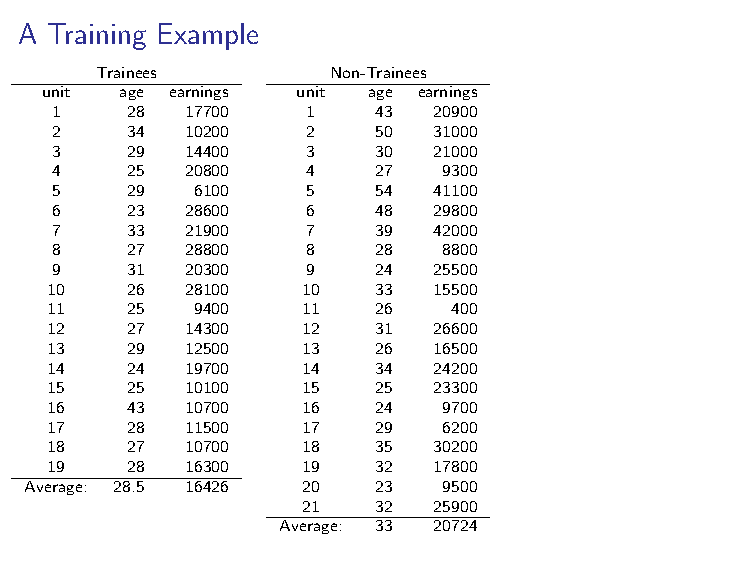
\includepdf[pages=1-last]{./lecture_includes/abadie-matching2.pdf}
}


\begin{frame}{Alternative distance metric: Euclidean distance}
	
 When the vector of matching covariates, $X= \colvec{X_1\\X_2\\\vdots\\X_k}$ has more than one dimension ($k>1$) we will need a new definition of \textbf{distance} to measure ``closeness''.  
\end{frame}

\begin{frame}{Alternative distance metric: Euclidean distance}
	\begin{block}{Definition: Euclidean distance}
    \vspace*{-2.5mm}
    \begin{eqnarray*}
    ||X_i-X_j|| &=& \sqrt{ (X_i-X_j)'(X_i-X_j) } \\
    &=& \sqrt{ \sum_{n=1}^k (X_{ni} - X_{nj})^2 }
    \end{eqnarray*}
    \vspace*{-2.5mm}
	\end{block}
	
  \textcolor{picton-blue}{Comment}: The Euclidean distance is not invariant to changes in the scale of the $X$'s.  For this reason, alternative distance metrics that \emph{are} invariant to changes in scale are used
	
\end{frame}


\begin{frame}{Normalized Euclidean distance}

	\begin{block}{Definition: Normalized Euclidean distance}
	  A commonly used distance is the normalized Euclidean distance:$$||X_i-X_j|| = \sqrt{ (X_i-X_j)'\widehat{V}^{-1}(X_i - X_j) }$$ where
		$$\widehat{V}^{-1} = \text{diag}(\widehat{\sigma}_1^2, \widehat{\sigma}_2^2, \dots, \widehat{\sigma}_k^2)$$
	\end{block}
\end{frame}

\begin{frame}{Normalized Euclidean distance}
	\begin{itemize}
	\item Notice that the normalized Euclidean distance is equal to:
		\begin{eqnarray*}
		||X_i - X_j|| = \sqrt{\sum_{n=1}^k \frac{(X_{ni} - X_{nj})}{\widehat{\sigma}^2_n}}
		\end{eqnarray*}
	\item Thus, if there are changes in the scale of $X_{ni}$, these changes also affect $\widehat{\sigma}^2_n$, and the normalized Euclidean distance does not change
	\end{itemize}

\end{frame}


\begin{frame}{Mahalanobis distance}
	
	\begin{block}{Definition: Mahalanobis distance}
	The Mahalanobis distance is the scale-invariant distance metric:
		\begin{eqnarray*}
		||X_i-X_j|| = \sqrt{ (X_i-X_j)'\widehat{\Sigma}_X^{-1}(X_i - X_j) }
		\end{eqnarray*}
	where $\widehat{\Sigma}_X$ is the sample variance-covariance matrix of $X$.
	\end{block}


\end{frame}


\begin{frame}{Arbitrary weights}
	
	Or, you could just create your own arbitrary weights
		\begin{eqnarray*}
		||X_i-X_j|| = \sqrt{ \sum_{n=1}^k \omega_n \cdot (X_{ni} - X_{nj})^2}
		\end{eqnarray*}(with all $\omega_n\geq{0}$) so that we assign large $\omega_n$'s to those covariates that we want to match particularly well.

\end{frame}

\begin{frame}{Matching and the Curse of Dimensionality}
	
Dimensionality creates headaches for us in matching.
	\begin{itemize}
	\item \textcolor{red}{Bad news}: Matching discrepancies $||X_i-X_{j(i)}||$ tend to increase with $k$, the dimension of $X$
	\item \textcolor{blue}{Good news}: Matching discrepancies converge to zero \dots
	\item \textcolor{red}{Bad news}: \dots but they converge very slow if $k$ is large
	\item \textcolor{blue}{Good news}: Mathematically, it can be shown that $||X_i-X_{j(i)}||$ converges to zero at the same rate as $\frac{1}{N^{\frac{1}{k}}}$
	\item \textcolor{red}{Bad news}: It's hard to find good matches when $X$ has a large dimension:  you need many observations if $k$ is big.
	\end{itemize}
\end{frame}


\begin{frame}{Deriving the matching bias}
	
  \vspace{-5mm}
  $$
		\widehat{\delta}_{ATT} = \frac{1}{N_T} \sum_{D_i=1} (Y_i - Y_{j(i)}),
  $$
  where each $i$ and $j(i)$ units are matched, $X_i \approx X_{j(i)}$ and $D_{j(i)}=0$. 
	 
  \bigskip
  Define potential outcomes and switching eq.
		\begin{eqnarray*}
      \mu^0(x) &=& E[Y | X=x,D=0] = E[Y^0 | X=x],\\
      \mu^1(x) &=& E[Y | X=x,D=1] = E[Y^1 | X=x],\\
      Y_i &=& \mu^{D_i}(X_i) + \varepsilon_i
		\end{eqnarray*}
\end{frame}

\begin{frame}{Deriving the matching bias}
  Substitute and distribute terms
  \begin{eqnarray*}
    \widehat{\delta}_{ATT} &=& \frac{1}{N_T} \sum_{D_i=1} (Y_i - Y_{j(i)}) \\
    &=& \frac{1}{N_T} \sum_{D_i=1} \left[ (\mu^1(X_i) + \varepsilon_i) - (\mu^0(X_{j(i)}) + \varepsilon_{j(i)}) \right] \\
    &=&  \frac{1}{N_T} \sum_{D_i=1} (\mu^1(X_i) - \mu^0(X_{j(i)})) + \frac{1}{N_T} \sum_{D_i=1}(\varepsilon_i - \varepsilon_{j(i)})
  \end{eqnarray*}
\end{frame}
		

\begin{frame}{Deriving the matching bias}
	
Difference between sample estimate and population parameter is:
		\begin{eqnarray*}
		\widehat{\delta}_{ATT} - \delta_{ATT} &=& \frac{1}{N_T} \sum_{D_i=1} \left( \mu^1(X_i) - \mu^0(X_{j(i)}) - \delta_{ATT}\right) \\
		&+& \frac{1}{N_T} \sum_{D_i=1} (\varepsilon_i - \varepsilon_{j(i)})
		\end{eqnarray*}
Algebraic manipulation and simplification:
		\begin{eqnarray*}
		\widehat{\delta}_{ATT} - \delta_{ATT} &=& \frac{1}{N_T} \sum_{D_i=1} \left( \mu^1(X_i) - \mu^0(X_i) - \delta_{ATT}\right) \\
		&+& \frac{1}{N_T} \sum_{D_i=1} (\varepsilon_i - \varepsilon_{j(i)}) \\
		&+& \frac{1}{N_T} \sum_{D_i=1} \left( \mu^0(X_i) - \mu^0(X_{j(i)}) \right).
		\end{eqnarray*}
\end{frame}


\begin{frame}{Deriving the matching bias}
	
Note $\widehat{\delta}_{ATT} - \delta_{ATT} \to 0$ as $N \to \infty$.
\pause However, 
$$E[ \sqrt{\frac{1}{N}} (\widehat{\delta}_{ATT} - \delta_{ATT})] = E[ \sqrt{\frac{1}{N}} ( \mu^0(X_i) - \mu^0(X_{j(i)}) ) | D=1].$$ 

Now consider the implications if $k$ is large:
	\begin{itemize}
	\item The difference between $X_i$ and $X_{j(i)}$ converges to zero very slowly
	\item The difference $\mu^0(X_i) - \mu^0(X_{j(i)})$ converges to zero very slowly
	\item $E[ \sqrt{\frac{1}{N}} (\mu^0(X_i) - \mu^0(X_{j(i)})) | D=1]$ may not converge to zero and an be very large!
	\item $E[ \sqrt{\frac{1}{N}} (\widehat{\delta}_{ATT} - \delta_{ATT})]$ may not converge to zero because the bias of the matching discrepancy is dominating the matching estimator!
	\end{itemize}
Bias is often an issue when we match in many dimensions
\end{frame}

\begin{frame}{Solutions to matching bias problem}
	
The bias of the matching estimator is caused by large matching discrepancies $||X_i - X_{j(i)}||$. The curse of dimensionality virtually guarantees this.  However:
	\begin{enumerate}
	\item But the matching discrepancies are observed. We can always check in the data how well we're matching the covariates.

	\item For $\widehat{\delta}_{ATT}$ we can sometimes make the matching discrepancies small by using a large reservoir of untreated units to select the matches (that is, by making $N_C$ large).

  \item If the matching discrepancies are large, so we are worried about potential biases, we can apply bias correction techniques

	\end{enumerate}
\end{frame}


\begin{frame}{Matching with bias correction}
	
	\begin{itemize}
	\item Each treated observation contributes$$\mu^0(X_i) - \mu^0(X_{j(i)})$$to the bias.
	\item Bias-corrected (BC) matching:
		\begin{eqnarray*}
		\widehat{\delta}_{ATT}^{BC} = \frac{1}{N_T} \sum_{D_i=1} \left[ (Y_i - Y_{j(i)}) - ( \widehat{\mu^0}(X_i) - \widehat{\mu^0}(X_{j(i)}) ) \right]
		\end{eqnarray*}where $\widehat{\mu^0}(X)$ is an estimate of $E[Y|X=x,D=0]$.  For example using OLS.  
	\item Under some conditions, the bias correction eliminates the bias of the matching estimator without affecting the variance.
	\end{itemize}
\end{frame}




\begin{frame}[plain,shrink=0]
	\begin{center}
	\textbf{Bias adjustment in matched data}
	\end{center}
	
	\begin{table}
	\begin{tabular}{c|c|c|c|c}
	\hline
	\multicolumn{1}{c}{}&
	\multicolumn{2}{c}{Potential Outcome}&
	\multicolumn{1}{c}{}&
	\multicolumn{1}{c}{}\\
	\multicolumn{1}{c}{unit} &
	\multicolumn{1}{c}{under Treatment}&
	\multicolumn{1}{c}{under Control}&
	\multicolumn{1}{c}{}&
	\multicolumn{1}{c}{}\\
	\hline
	$i$ & $Y^1_i$ & $Y^0_i$ & $D_i$ & $X_i$ \\
	\hline
	1 & \textcolor{blue}{10} &  \textcolor{blue}{8} & 1 & \textcolor{blue}{3} \\
	2 & 4 &  			 1 &				 1 & 1 \\
	3 & \textcolor{green}{10} &   \textcolor{green}{9} & 1 & \textcolor{green}{10} \\
	\hline
	4 &  & \textcolor{blue}{8} & 0 & \textcolor{green}{4} \\
	5 &  & 			 1 & 0 &  				0 \\
	6 &  & \textcolor{green}{9} & 0 & \textcolor{green}{8} \\
	\hline
	\end{tabular}
	\end{table}
	
	
	\begin{flalign*}
		\only<1-3>{&\widehat{\delta}_{ATT} = \frac{10-8}{3} + \frac{4-1}{3}  + \frac{10-9}{3}  = 2&} \\
		\only<2-3>{&\text{For the bias correction, estimate }\widehat{\mu^0}(X) = \widehat{\beta_0} + \widehat{\beta_1}X = 2+X}\\
		\only<3-3>{&\widehat{\delta}_{ATT} = \frac{ (10-8) - ( \widehat{\mu^0}(3) - \widehat{\mu^0}(4)) }{3}  + \frac{ (4-1)  -( \widehat{\mu^0}(1) - \widehat{\mu^0}(0)) }{3}  \\
		&+ \frac{ (10-9)  - ( \widehat{\mu^0}(10) - \widehat{\mu^0}(8))}{3} = 1.33}
	\end{flalign*}

\end{frame}


\begin{frame}{Matching bias: Implications for practice}
	
Bias arises because of the effect of large matching discrepancies on $\mu^0(X_i) - \mu^0(X_{j(i)})$. To minimize matching discrepancies:
	\begin{enumerate}
	\item Use a small $M$ (e.g., $M=1$). Larger values of $M$ produce large matching discrepancies.
	\item Use matching with replacement.  Because matching with replacement can use untreated units as a match more than once, matching with replacement produces smaller matching discrepancies than matching without replacement.
	\item Try to match covariates with a large effect on $\mu^0(\cdot)$ particularly well.
	\end{enumerate}
\end{frame}

\begin{frame}{Large sample distribution for matching estimators}
	
	\begin{itemize}
	\item Matching estimators have a Normal distribution in large samples (provided the bias is small):
		\begin{eqnarray*}
		\sqrt{N_T} (\widehat{\delta}_{ATT} - \delta_{ATT}) \xrightarrow{d} N(0,\sigma^2_{ATT})
		\end{eqnarray*}
	\item For matching without replacement, the ``usual'' variance estimator:
		\begin{eqnarray*}
		\widehat{\sigma}^2_{ATT} = \frac{1}{N_T} \sum_{D_i=1} \left( Y_i - \frac{1}{M} \sum_{m=1}^M Y_{j_m(i)} - \widehat{\delta}_{ATT} \right)^2,
		\end{eqnarray*}is valid.
	\end{itemize}
\end{frame}

\begin{frame}{Large sample distribution for matching estimators}
	
	\begin{itemize}
	\item For matching with replacement:
		\begin{eqnarray*}
		\widehat{\sigma}^2_{ATT} &=& \frac{1}{N_T} \sum_{D_i=1} \left( Y_i - \frac{1}{M} \sum_{m=1}^M Y_{j_m(i)} - \widehat{\delta}_{ATT} \right)^2 \\
		&+& \frac{1}{N_T} \sum_{D_i=0} \left( \frac{K_i(K_i-1)}{M^2} \right) \widehat{var}(\varepsilon | X_i,D_i=0)
		\end{eqnarray*}where $K_i$ is the number of times observation $i$ is used as a match.
	\item $\widehat{var}(Y_i | X_i,D_i=0)$ can be estimated also by matching.  For example, take two observations with $D_i=D_j=0$ and $X_i \approx X_j$, then
		\begin{eqnarray*}
		\widehat{var}(Y_i | X_i,D_i=0) = \frac{(Y_i-Y_j)^2}{2}
		\end{eqnarray*}is an unbiased estimator of $\widehat{var}(\varepsilon_i | X_i,D_i=0))$
	\end{itemize}
\end{frame}
	

		  
\subsection{Propensity scores}

\begin{frame}{Avoiding dimensionality problems}
	
	\begin{itemize}
	\item Curse of dimensionality makes matching on $K$ covariates challenging
	\item Rubin (1977) and Rosenbaum and Rubin (1983) develop a method that can contain those $K$ covariates used for adjusting
	\item Insofar as treatment is random conditional on $K$ covariates, then one can use the propensity score to adjust for confounders 
	\end{itemize}
	
\end{frame}



\begin{frame}{Least squares}
	
	\begin{itemize}
	\item OLS is best linear predictor and approximation to the conditional expectation function 
	\item But if probability of treatment is nonlinear, this conditional mean may be less informative
	\item Propensity scores relax the linearity assumption and have other advantages
	\end{itemize}
\end{frame}



\begin{frame}{The Idea behind propensity scores}
	
	\begin{itemize}
	\item Earlier we matched on $X$'s to compare units ``near'' one another based on some distance but matching discrepancies and sparseness created problems
	\item Propensity scores summarize covariate information about treatment selection into a single number bounded between 0 and 1 (i.e., a probability)
	\item Now we compare units with similar \emph{estimated probabilities} of treatment
	\item And once we adjust using the propensity score, we no longer need to adjust for $X$
	\end{itemize}
\end{frame}



\begin{frame}{Formal Definition}
	
	\begin{block}{Definition of Propensity score}
	A propensity score is a number bounded between 0 and 1 measuring the probability of treatment assignment conditional on a vector of confounding variables: $p(X)=Pr(D=1 | X)$
	\end{block}
	
	Two Necessary Identification Assumptions:
	\begin{enumerate}
	\item $(Y^0,Y^1) \independent{D}|X$ (CIA)
	\item $0<Pr(D=1|X)<1$ (common support)
	\end{enumerate}

\end{frame}


\begin{frame}{Steps}
	
		\begin{enumerate}
		\item Estimate the propensity score using logit/probit
		\item Estimate a particular ATE incorporating the propensity score using stratification, imputation, regression, or inverse probability weighting
		\item Estimate standard errors
		\end{enumerate}
\end{frame}

\begin{frame}{Estimating the propensity score}

		\begin{itemize}
		\item Estimate the conditional probability of treatment using probit or logit model$$Pr(D_i=1|X_i) = F(\beta X_i)$$
		\item Use the estimated coefficients to calculate the propensity score for each unit $i$$$\widehat{\rho}_i = \widehat{\beta} X_i$$
		\item Propensity score is the predicted conditional probability of treatment, or the fitted value for each unit -- it is the likelihood you'd be in the treatment group given your covariates
		\item Frequentist probability in other words
		\end{itemize}
\end{frame}

\begin{frame}{Identification}
	
	\begin{itemize}
	\item A group of unit's average treatment effect may depend on some characteristic, $X$
		\begin{eqnarray*}
		E[\delta_i(X_i) ]&=& E[Y^1_i - Y^0_i | X_i=x] \\
		&=&E[Y^1_i | X_i=x] - E[Y^0_i | X_i=x]
		\end{eqnarray*}
	\item CIA allow us to substitute $$E[Y_i | D_i =1, X_i=x]=E[Y_i^1 | D_i=1, X_i=x]$$ and similar for other term $Y^0$ using a switching equation
	\item Common support allows us to estimate both terms
	\end{itemize}
\end{frame}		


\begin{frame}[plain]
	
	\begin{block}{Propensity score theorem}
	If $(Y^1,Y^0)\independent{D}|X$ (CIA), then $(Y^1,Y^0)\independent{D} | \rho(X)$ where $\rho(X)=Pr(D=1|X)$, the propensity score
	\end{block}
	
	\begin{itemize}
	\item Conditioning on the propensity score is enough to have independence between $D$ and $(Y^1,Y^0)$ (Rosenbaum and Rubin 1983)\\
	 \item Valuable theorem because of dimension reduction and convergence rate issues which can introduce biases
	\item \textbf{Big picture}: You can toss $X$ out if you have $\widehat{\rho}$ because all information from $X$ have been absorbed into $\widehat{\rho}$
	\end{itemize}
\end{frame}

\begin{frame}{Proof}
	
	\begin{itemize}
	\item Before diving into the proof, first recognize that$$Pr(D=1|Y^0,Y^1\rho(X)) = E[D | Y^0,Y^1,\rho(X)]$$because
		\begin{eqnarray*}
		E[D|Y^0,Y^1,\rho(X)] &=& 1\times Pr(D=1|Y^0,Y^1,\rho(X)) \\
		& & + 0 \times Pr(D=0 | Y^0,Y^1,\rho(X))
		\end{eqnarray*}and the second term cancels out.
		\end{itemize}
\end{frame}

\begin{frame}[plain,shrink=5]
	
	\begin{proof}
	Assume $(Y^1,Y^0)\independent{D}|X$ (CIA).  Then:
		\begin{eqnarray*}
		Pr(D=1 | Y^1,Y^0, \rho(X)) &=& \underbrace{\textcolor{blue}{E[D | Y^1, Y^0, \rho(X)]}}_{ \mathclap{\text{See previous slide}}} \\
		&=&\underbrace{\textcolor{blue}{E} [ E [ D | Y^1,Y^0, \rho(X), X] \textcolor{blue}{| Y^1,Y^0,\rho(X)]}}_{ \mathclap{\text{by LIE}}} \\
		&=&\underbrace{\textcolor{blue}{E} [ E [ D | Y^1,Y^0,X] \textcolor{blue}{| Y^1,Y^0,\rho(X)]}}_{ \mathclap{\text{Given $X$, we know $p(X)$}}} \\
		&=&\underbrace{\textcolor{blue}{E} [E [D | X] \textcolor{blue}{| Y^1,Y^0,\rho(X)]}}_{ \mathclap{\text{by CIA}}} \\
		&=& \underbrace{\textcolor{blue}{E}[\rho(X) \textcolor{blue}{| Y^1, Y^0, \rho(X)]}}_{ \mathclap{\text{propensity score definition}}} \\
		&=& \rho(X)
		\end{eqnarray*}
	\end{proof}
	
\end{frame}

\begin{frame}{Similar proof}

	 We also can show that the probability of treatment conditional on the propensity score is the propensity score using a similar argument:
		\begin{eqnarray*}
		Pr(D=1| \rho(X)) &=& \underbrace{E[ D | \rho(X) ]}_{\mathclap{\text{Previous slide}}} \\
		&=& \underbrace{E [ E [D | X] | \rho(X)]}_{ \mathclap{\text{LIE}}} \\
		&=& \underbrace{E[p(X) | \rho(X)]}_{ \mathclap{\text{definition}}} \\
		&=& \rho(X)
		\end{eqnarray*}and $Pr(D=1 | Y^1, Y^0, \rho(X)) = Pr(D=1| \rho(X))$ by CIA
\end{frame}


\begin{frame}{Unbiased estimation of the ATE}

Exact methods to do this to be discussed later, but until then, we can say this:
	\begin{block}{Corollary: Estimating the ATE}
	If $(Y^1,Y^0)\independent{D}|X$, we can estimate average treatment effects:
 $$E[Y^1-Y^0|\rho(X)] = E[Y|D=1,\rho(X)] - E[Y|D=0,\rho(X)]$$
	\end{block}
	
\end{frame}

\begin{frame}{Balancing property}
	
	\begin{itemize}
	\item Because the propensity score is a function of X, we know:
		\begin{eqnarray*}
		Pr(D=1 | X,\rho(X)) &=& Pr(D=1|X)\\
		&=& \rho(X)
		\end{eqnarray*}
	\item Conditional on $\rho(X)$, the probability that $D=1$ does not depend on $X$.  
	\item $D$ and $X$ are independent conditional on $p(X)$: $$D\independent{X} | \rho(X)$$
	\end{itemize}
\end{frame}


\begin{frame}{Balancing property}

\begin{itemize}
	\item So we obtain the \textbf{balancing property} of the propensity score: $$Pr(X|D=1,p(X)) = Pr(X|D=0, p(X))$$ conditional on the property score, the distribution of the covariates is the same for treatment and control group units
	\item We can use this to check if our estimated propensity score actually produces balance:$$Pr(X|D=1,\widehat{p}(X)) = Pr(X|D=0, \widehat{p}(X))$$
\end{itemize}

\end{frame}


\begin{frame}{Propensity score theorem}
	
	\begin{itemize}
	\item This theorem tells us the \emph{only} covariate we need to adjust for is the conditional probability of treatment itself (i.e., the propensity score)
	\item It does not tell us which method we should use to do that adjustment, though, which is an estimation question
	\item There are options: inverse probability weighting, forms of imputation, stratification, and sometimes even regressions will incorporate the score as weights
	\end{itemize}
\end{frame}



\begin{frame}{Checking the common support assumption}
	
	\begin{itemize}
	\item We can summarize the propensity scores in the treatment and control group and count how many units are off-support
	\item Crump, et al. (2009) offer a rule of thumb: keep scores on interval [0.1,0.9]. 
	\item Tossing out observations beyond those min and max scores
	\item A histogram of propensity scores by treatment and control group also highlights the overlap problem; software also can help such as \texttt{teffects overlap}
	\end{itemize}
	
\end{frame}



\subsection{Inverse probability weighting}

\begin{frame}{Inverse probability weighting}

\begin{itemize}
	\item I really like the simple method of inverse probability weighting aesthetically because there are no black boxes; it's all non-parametric averaging done through a particular kind of weights based on the propensity score
	\item IPW involves fewer implementation choices like number of neighbors, common support, etc.
	\item And because IPW is a smooth estimator, the bootstrap is valid for inference unlike covariate nearest neighbor matching which Abadie and Imbens (2008) show is not valid
\end{itemize}

\end{frame}

\begin{frame}{Inverse probability weighting}

\begin{itemize}
	\item IPW is basically a reweighting of the outcomes by the propensity score developed in Robins and Rotnitzky (1995), Imbens (2000), Hirano and Imbens (2001)
	\item The weights can be expressed in two ways -- without normalization (Horvitz and Thompson 1952) or normalized (Hajek1971) -- the difference being how well either approach can handle extreme values of the propensity score; the differences come out of the survey sampling literature 
	\item Notation is far far scarier than in fact what we are doing, so I'll show you this in a Stata and R simulation to help pin down the intuition a little better
	\item We'll start with the basic idea using the Horvitz and Thompson (1952) expression of the weights as it's not as messy.
\end{itemize}

\end{frame}
	
	

\begin{frame}{Inverse Probability Weighting}
	
		\begin{block}{Proposition}
	If $Y^1,Y^0 \independent{D}|X$, then
		\begin{eqnarray*}
		\delta_{ATE}&=&E[Y^1-Y^0] \\
		&=&E \left[ Y \cdot  \frac{D - \rho(X)}{\rho(X) \cdot (1-\rho(X))} \right]\\
		\delta_{ATT}&=&E[Y^1-Y^0|D=1] \\
		&=& \frac{1}{Pr(D=1)} \cdot  E \left[ Y \cdot \frac{D-\rho(X)}{1-\rho(X)} \right]
		\end{eqnarray*}
	\end{block}

\end{frame}

\begin{frame}[plain,shrink=5]
\begin{center}
\textbf{IPW Proof}
\end{center}

	\begin{proof}
	\begin{eqnarray*}
	E \left[ Y \cdot \frac{D-\rho(X)}{\rho(X)(1-\rho(X))} \Big\vert X \right] &=& E \left[ \frac{Y}{\rho(X)} \Big\vert X,D=1 \right] \rho(X) \\
	&& + E\left[ \frac{-Y}{1-\rho(X)} \Big\vert X,D=0 \right](1-\rho(X)) \\
	&=& E[Y|X,D=1] - E[Y|X,D=0]
	\end{eqnarray*}and the results follow from integrating over $P(X)$ and $P(X|D=1)$.
	\end{proof}

\end{frame}


\begin{frame}{Weighting on the propensity score}

Previous formulas used population concepts. Switching to samples, we use a two-step estimator:
	\begin{enumerate}
	\item Estimate the propensity score: $\widehat{\rho}(X)$
	\item Use estimated score to produce analog estimators. Let $\widehat{\delta}_{ATE}$ and $\widehat{\delta}_{ATT}$  be an estimate of the $ATE$ and $ATT$ parameter:
		\begin{eqnarray*}
		\widehat{\delta}_{ATE} &=& \frac{1}{N} \sum_{i=1}^N Y_i \cdot \frac{D_i - \widehat{\rho}(X_i)}{\widehat{\rho}(X_i) \cdot (1-\widehat{\rho}(X_i))}\\
		\widehat{\delta}_{ATT} &=& \frac{1}{N_T} \sum_{i=1}^N Y_i \cdot \frac{D_i - \widehat{\rho}(X_i)}{1-\widehat{\rho}(X_i)}
		\end{eqnarray*}
	\end{enumerate}
\end{frame}

\begin{frame}{Weighting on the propensity score}
	
		
Standard errors can be constructed a few different ways:
	\begin{itemize}
	\item We need to adjust the standard errors for first-step estimation of $\rho(X)$
	\item Parameteric first step: Newey and McFadden (1994)
	\item Non-parametric first step: Newey (1994)
	\item Or bootstrap the entire two-step procedure (Adudumilli 2018 and Bodory et al. 2020)
	\end{itemize}
\end{frame}



\begin{frame}{Implementation with software}

\begin{itemize}
\item I like estimating with IPW manually because I like being reminded how simple a procedure it is
\item But Stata's -teffects- and R's -ipw- do it too, and -teffects- uses the Hajek normalization weights which will produce identical estimates to my program
\item My programs don't do the inference, but I think that would be fun and easy to do using the bootstrap
\item Let's look at it real quickly now with an example from LaLonde's 1986 paper on the NSW job trainings program (which I'll discuss again soon)
\end{itemize}

\end{frame}

\subsubsection{Double robust}
\begin{frame}{Double robust estimators}

\begin{itemize}
\item Lots of papers: Robins and Rotnizky (1995) originally, Hirano and Imbens (2001), etc.
\item Basic idea is you are going to control for covariates twice: through regression and then through the propensity score
\item We say that estimators combining regression with IPW are double robust so long as
	\begin{itemize}
	\item The regression for the outcome is properly specified, or
	\item The propensity score is properly specified
	\end{itemize}
\item Hence the name ``double robust''. We give ourselves two chances to get it right (either/or not both/and)
\end{itemize}

\end{frame}

\begin{frame}{Estimation of outcome model}

\begin{eqnarray*}
y_i = \alpha_0 + X_i\beta + \tilde{\alpha_1} D_i + \theta_0 \frac{D_i}{\widehat{\rho (X_i)}} + \theta_1 \frac{1-D_i}{1- \widehat{\rho (X_i)}} + \tilde{\varepsilon_i}
\end{eqnarray*}

\end{frame}

\subsection{Propensity score matching}

\begin{frame}

	\begin{center}
	\textbf{Propensity score matching}
	\end{center}
	
	\begin{itemize}
	\item Matching, or what I like to call ``imputation'', is another way that utilizes the $\widehat{\rho}$
	\item They all use the same first stage, but differ on their second and third stages
	\item Part of the second stage may be imposing common support through ``trimming'', but for different reasons because now this idea of distance is entering and maybe you think some units are ``too far away'' to be relevant counterfactuals
	\end{itemize}

\end{frame}




\begin{frame}{Standard matching strategy}
	
	\begin{itemize}
	\item Pair each treatment unit $i$ with one or more \emph{comparable} control group unit $j$, where comparability is in terms of proximity to the estimated propensity score
	\item Impute the unit's missing counterfactual outcome $Y_{i(j)}$ based on the unit or units chosen in the previous step
	\item If more than one are ``nearest neighbors'', then use the neighbors' weighted outcomes  $$Y_{i(j)} = \sum_{j \in C(i)} w_{ij}Y_j$$ where $C(i)$ is the set of neighbors with $W=0$ of the treatment unit $i$and $w_{ij}$ is the weight of control group units $j$ with $\sum_{j \in C(i)} w_{ij} = 1$
	\end{itemize}
\end{frame}


\begin{frame}{Imputing the counterfactuals}
	
	A parameter of interest: $$E[Y^1_i | D_i=1] - E[Y^0_i | D_i=1]$$We estimate it as follows  $$\widehat{ATT} = \frac{1}{N_T} = \sum_{i:W_i=1} \bigg [Y_i - Y_{i(j)} \bigg ]$$where $N_T$ is the number of matched treatment units in the sample. Note the difference between \emph{imputation} and weighting

\end{frame}

\begin{frame}{Matching methods}
	
	\begin{itemize}
	\item The probability of observing two units with \emph{exactly} the same propensity score is in principle zero because $p(x)$ is continuous
	\item Several matching methods have been proposed in the literature, but the most widely used are:
		\begin{itemize}
		\item Stratification matching
		\item Nearest-neighbor matching (with or without caliper)
		\item Radius matching
		\item Kernel matching
		\end{itemize}
	\item Typically, one treatment unit $i$ is matched to several control units $j$, but sometimes one-to-one matching is used
	\end{itemize}
	
\end{frame}


\begin{frame}{Stratification}
	
	\begin{itemize}
	\item Stratification is used to force covariate balance by finding strata where there is no difference in mean covariate values. 
	\item You then use those strata to calculate within differences in means and sum over properly weighted strata. See Becker and Ichino (2002)
	\item  Stratification is a brute force method for imposing balance by grouping the data and testing for differences in covariate means
	\item It's actually kind of similar to coarsened exact matching, only using the propensity score for the ``stratification'' not the covariates
	\end{itemize}
	
\end{frame}


\begin{frame}{Stratification: Achieving Balance}
	
The algorithm is brute force covariate balancing
	\begin{enumerate}
		\item Sort the data by propensity score and divide into groups of observations with similar propensity scores (e.g., percentiles)
		\item Within each group, test (using a t-test) whether the means of the covariates ($X$) are equal between treatment and control
		\item If so, then stop.  If not, it means the covariates aren't balanced \emph{within that group}.  Divide the group in half and repeat
		\item If a particular covariate is unbalanced for multiple groups, modify the initial logit or probit equation by including higher order terms and/or interactions with that covariate and repeat
		\end{enumerate}
Historically this could be done with -\texttt{pscore2.ado}- or manually oneself if they felt so inclined, but it was dropped with -\texttt{teffects}-
\end{frame}


\begin{frame}{Nearest Neighbor}
	
	Pretty similar to covariate matching.  Formula is $$ATT^{NN} = \frac{1}{N_T} \sum_{i:W_i=1} \bigg [ Y_i - \sum_{j \in C(i)_M} w_{ij}Y_j \bigg ]$$ 
		\begin{itemize}
		\item $N_T$ is the number of Treatment units $i$
		\item $w_{ij}$ is equal to $\frac{1}{N_C}$ if $j$ is a control unit and zero otherwise; $N_C$ is number of control units $j$
		\item And unit $j$ is chosen as a control for $i$ if it's propensity score is nearest to that of $i$
		\end{itemize}
\end{frame}

\begin{frame}[plain]
	
	\begin{center}
	\textbf{NN Matching: Bias vs. Variance}
	\end{center}
	
	\begin{itemize}
	\item But how far away on the propensity score will you use? Herein lies the different types of matching proposed
		\begin{itemize}
		\item Matching just one nearest neighbor minimizes bias at the cost of larger variance
		\item Matching using additional nearest neighbors increases the bias but decreases the variance
		\end{itemize}
	\item Matching with or without replacement
		\begin{itemize}
		\item with replacement keeps bias low at the cost of larger variance
		\item without replacement keeps variance low but at the cost of potential bias
		\end{itemize}
	\end{itemize}
	
\end{frame}


\begin{frame}{Distance between treatment and control units}

\begin{itemize}
\item What was historically done was limiting ``distance''  through various \emph{ad hoc} choices
\item Imagine these choices as creating like a lasso (like the cowboy rope)
\item Anything within the lasso could be used for the imputation; anything outside the lasso could not
\item There were two common ways -- caliper matching and radius matching. 
\end{itemize}

\end{frame}

\begin{frame}{Caliper matching}
	
	\begin{itemize}
	\item Caliper matching is a variation on NN matching that tries to build brakes into the algorithm as to avoid ``bad neighbors''
	\item It does this by imposing a tolerable maximum distance (e.g., 0.2 units in the propensity score away from a treatment unit $i$'s propensity score)
	\item Note -- this is a one-to-one imputation, and if there doesn't exist anybody in the control group unit $j$ within that ``caliper'', then treatment unit $i$ is discarded
	\item Means we aren't estimating the ATE anymore once we start dropping units
	\item It's difficult to know what this caliper should be \emph{ex ante}, hence why I said it is somewhat \emph{ad hoc}
	\end{itemize}

\end{frame}


\begin{frame}{Radius matching}
	
	
		\begin{itemize}
		\item Each treatment unit $i$ is matched with the control group units whose propensity score are in a predefined neighborhood of the propensity score of the treatment unit.
		\item \textbf{All} the control units with $\widehat{\rho_j}$ falling within a radius $r$ from $\widehat{\rho}_i$ are matched to the treatment unit $i$ -- this is what distinguishes it from calipers, and makes it more similar to covariate matching (Abadie and Imbens 2006, 2008)
		\item The smaller the radius, the better the quality of the matches, but the higher the possibility some treatment units are not matched because the neighborhood does not contain control group units $j$
		\end{itemize}
		
\end{frame}

\begin{frame}{Software}

\begin{itemize}
\item I think you can use -\texttt{teffects, psmatch}- to get at these two nearest neighbor approaches by setting the number of matches
\item You can use -\texttt{pscore2}- for stratification, but I think the standard errors are wrong, so you may need to just do it manually using bootstrapping or variance approximation, and that may be a pain to program up
\item Not sure of the R command, but I know it's out there
\end{itemize}

\end{frame}


\begin{frame}{King and Nielsen (2019)}
	
	\begin{itemize}
	\item There is a King and Nielsen (2019) critique of these methods that is popularly known but not popularly studied
	\item King and Nielsen (2019) is not a critique of the propensity score, because it does not apply to stratification, regression adjustment, or inverse probability weighting
	\item It only applies to nearest neighbor and is related to forced balance through trimming and a myriad of other common choices made by the researcher
	\end{itemize}
	
\end{frame}

\begin{frame}[plain]

\begin{quote}
	

```[The] more balanced the data, or the more balance it becomes by [trimming] some of the observations through matching, the more likely propensity score matching will degrade inferences.'' -- King and Nielsen (2019)

\end{quote}
	
\end{frame}


\begin{frame}{Examples of propensity score matching}
	
	\begin{itemize}
	\item Workhorse example of propensity score matching is the Job Trainings Program (NSW) 
	\item First studied by LaLonde (1986) evaluating multiple econometric models for program evaluation 
		\begin{itemize}
		\item All the standard estimators failed to estimate the known ATE when replacing experimental controls with non-experimental controls -- even difference-in-differences
		\end{itemize}
	\item Dehejia and Wahba (1999; 2002) use LaLonde's data with propensity score matching and found better results
	\item Critiques by Petra Todd, Jeff Smith and others followed which I won't review here for sake of time
	\end{itemize}
\end{frame}



\begin{frame}{Description of NSW Job Trainings Program}
	
The National Supported Work Demonstration (NSW), operated by Manpower Demonstration Research Corp in the mid-1970s:
	\begin{itemize}
	\item was a temporary employment program designed to help disadvantaged workers lacking basic job skills move into the labor market by giving them work experience and counseling in a sheltered environment
	\item was also unique in that it \textbf{randomly assigned} qualified applicants to training positions:
		\begin{itemize}
		\item \textbf{Treatment group}: received all the benefits of NSW program
		\item \textbf{Control group}: left to fend for themselves
		\end{itemize}
	\item admitted AFDC females, ex-drug addicts, ex-criminal offenders, and high school dropouts of both sexes
	\end{itemize}
\end{frame}

\begin{frame}{NSW Program}
	
	\begin{itemize}
	\item Treatment group members were:
		\begin{itemize}
		\item guaranteed a job for 9-18 months depending on the target group and site
		\item divided into crews of 3-5 participants who worked together and met frequently with an NSW counselor to discuss grievances and performance
		\item paid for their work
		\end{itemize}
	\item Control group members were randomized so the same
	\item Note: the randomization balanced observables and unobservables across the two arms, thus enabling the estimation of an ATE for the people who self-selected into the program
	\end{itemize}
\end{frame}

\begin{frame}{NSW Program}

\begin{itemize}
	\item Other details about the NSW program:
		\begin{itemize}
		\item \underline{Wages}:  NSW offered the trainees lower wage rates than they would've received on a regular job, but allowed their earnings to increase for satisfactory performance and attendance
		\item \underline{Post-treatment}: after their term expired, they were forced to find regular employment
		\item \underline{Job types}:  varied within sites -- gas station attendant, working at a printer shop -- and males and females were frequently performing different kinds of work
		\end{itemize}
\end{itemize}

\end{frame}
	
\begin{frame}{NSW Data}
	
	\begin{itemize}
	\item \underline{NSW data collection}:
		\begin{itemize}
		\item MDRC collected earnings and demographic information from both treatment and control at baseline and every 9 months thereafter
		\item Conducted up to 4 post-baseline interviews
		\item Different sample sizes from study to study can be confusing, but has simple explanations
		\end{itemize}
	\end{itemize}
\end{frame}
	

\begin{frame}{NSW Data}

\begin{itemize}
	\item \underline{Estimation}:
		\begin{itemize}
		\item NSW was a randomized job trainings program; therefore estimating the average treatment effect is straightforward:
			\begin{eqnarray*}
			\frac{1}{N_t}\sum_{D_i=1}Y_i - \frac{1}{N_c}\sum_{D_i=0}Y_i \approx E[Y^1-Y^0] 
			\end{eqnarray*}in large samples assuming treatment selection is independent of potential outcomes (randomization) -- i.e., $(Y^0,Y^1)\independent{D}$. 
		\end{itemize}
	\item \underline{NSW worked}: Treatment group participants' real earnings post-treatment (1978) was positive and economically meaningful -- $\approx$ \$900 (LaLonde 1986) to \$1,800 (Dehejia and Wahba 2002) depending on the sample used
\end{itemize}

\end{frame}
	
\begin{frame}[plain]
	\begin{center}
	LaLonde, Robert J. (1986). \myurlshort{http://business.baylor.edu/scott_cunningham/teaching/lalonde-1986.pdf}{``Evaluating the Econometric Evaluations of Training Programs with Experimental Data''}. \emph{American Economic Review}. 
	\end{center}
	
\underline{LaLonde's study} was \textbf{not} an evaluation of the NSW program, as that had been done, but rather an evaluation of econometric models done by:
		\begin{itemize}
		\item replacing the experimental NSW control group with non-experimental control group drawn from two nationally representative survey datasets: Current Population Survey (CPS) and Panel Study of Income Dynamics (PSID)
		\item estimating the average effect using non-experimental workers as controls for the NSW trainees 
		\item comparing his non-experimental estimates to the experimental estimates of \$900
		\end{itemize}
\end{frame}

\begin{frame}{LaLonde (1986)}

\begin{itemize}

	\item \underline{LaLonde's conclusion}: available econometric approaches were biased and inconsistent
		\begin{itemize}
		\item His estimates were way off and usually the wrong sign
		\item Conclusion was influential in policy circles and led to greater push for more experimental evaluations
		\end{itemize}

\end{itemize}

\end{frame}

\imageframe{./lecture_includes/lalonde_table5a.png}
\imageframe{./lecture_includes/lalonde_table5b.png}

\begin{frame}[plain,shrink=10]{Imbalanced covariates for experimental and non-experimental samples}

    \begin{center}
		\begin{table}
		\begin{tabular}{lcccccc}
		\hline \hline
		\multicolumn{3}{c}{}&
		\multicolumn{1}{c}{CPS}&
		\multicolumn{1}{c}{NSW}\\
		
		\multicolumn{1}{c}{}&
		\multicolumn{2}{c}{All} &
		\multicolumn{1}{c}{Controls} &
		\multicolumn{1}{c}{Trainees} \\

		\multicolumn{3}{c}{}&
		\multicolumn{1}{c}{$N_c=15,992$}&
		\multicolumn{1}{c}{$N_t=297$}&
		\multicolumn{1}{c}{}&
		\multicolumn{1}{c}{}\\

		\multicolumn{1}{l}{covariate}&
		\multicolumn{1}{c}{mean}&
		\multicolumn{1}{c}{(s.d.)}&
		\multicolumn{1}{c}{mean}&
		\multicolumn{1}{c}{mean}&
		\multicolumn{1}{c}{t-stat}&
		\multicolumn{1}{c}{diff}\\
		\hline
Black    & 0.09 & 0.28 & 0.07 & 0.80 & 47.04 & -0.73\\
Hispanic & 0.07 & 0.26 & 0.07 & 0.94 & 1.47 & -0.02\\
Age & 33.07 & 11.04 & 33.2 & 24.63 & 13.37  & 8.6\\
Married & 0.70 & 0.46 & 0.71 & 0.17 & 20.54 & 0.54\\
No degree & 0.30 & 0.46 & 0.30 & 0.73 & 16.27 & -0.43\\
Education & 12.0 & 2.86 & 12.03 & 10.38 & 9.85 & 1.65 \\
1975 Earnings   & 13.51 & 9.31 & 13.65 & 3.1 & 19.63 & 10.6\\
1975 Unemp  & 0.11 & 0.32 & 0.11 & 0.37 & 14.29 & -0.26\\
		\hline 
		\end{tabular}
		\end{table}
    \end{center}

\end{frame}


\begin{frame}{Dehija and Wahba (1999)}
	
	\begin{itemize}
	\item Dehejia and Wahba (DW) update LaLonde's original study using propensity score matching
		\begin{enumerate}
		\item Dehejia, Rajeev H. and Sadek Wahba (1999). 	``Causal Effects in Nonexperimental Studies: Reevaluating the Evaluation of Training Programs''. \underline{Journal of the American Statistical} \underline{Association}, vol. 94(448): 1053-1062 (\myurlshort{http://business.baylor.edu/scott_cunningham/teaching/dehejia-and-wahba-1999.pdf}{pdf})
		\end{enumerate}
	\item Can propensity score matching improve over the estimators that LaLonde examined?
	\end{itemize}
\end{frame}

\begin{frame}[plain]
	
\begin{figure}
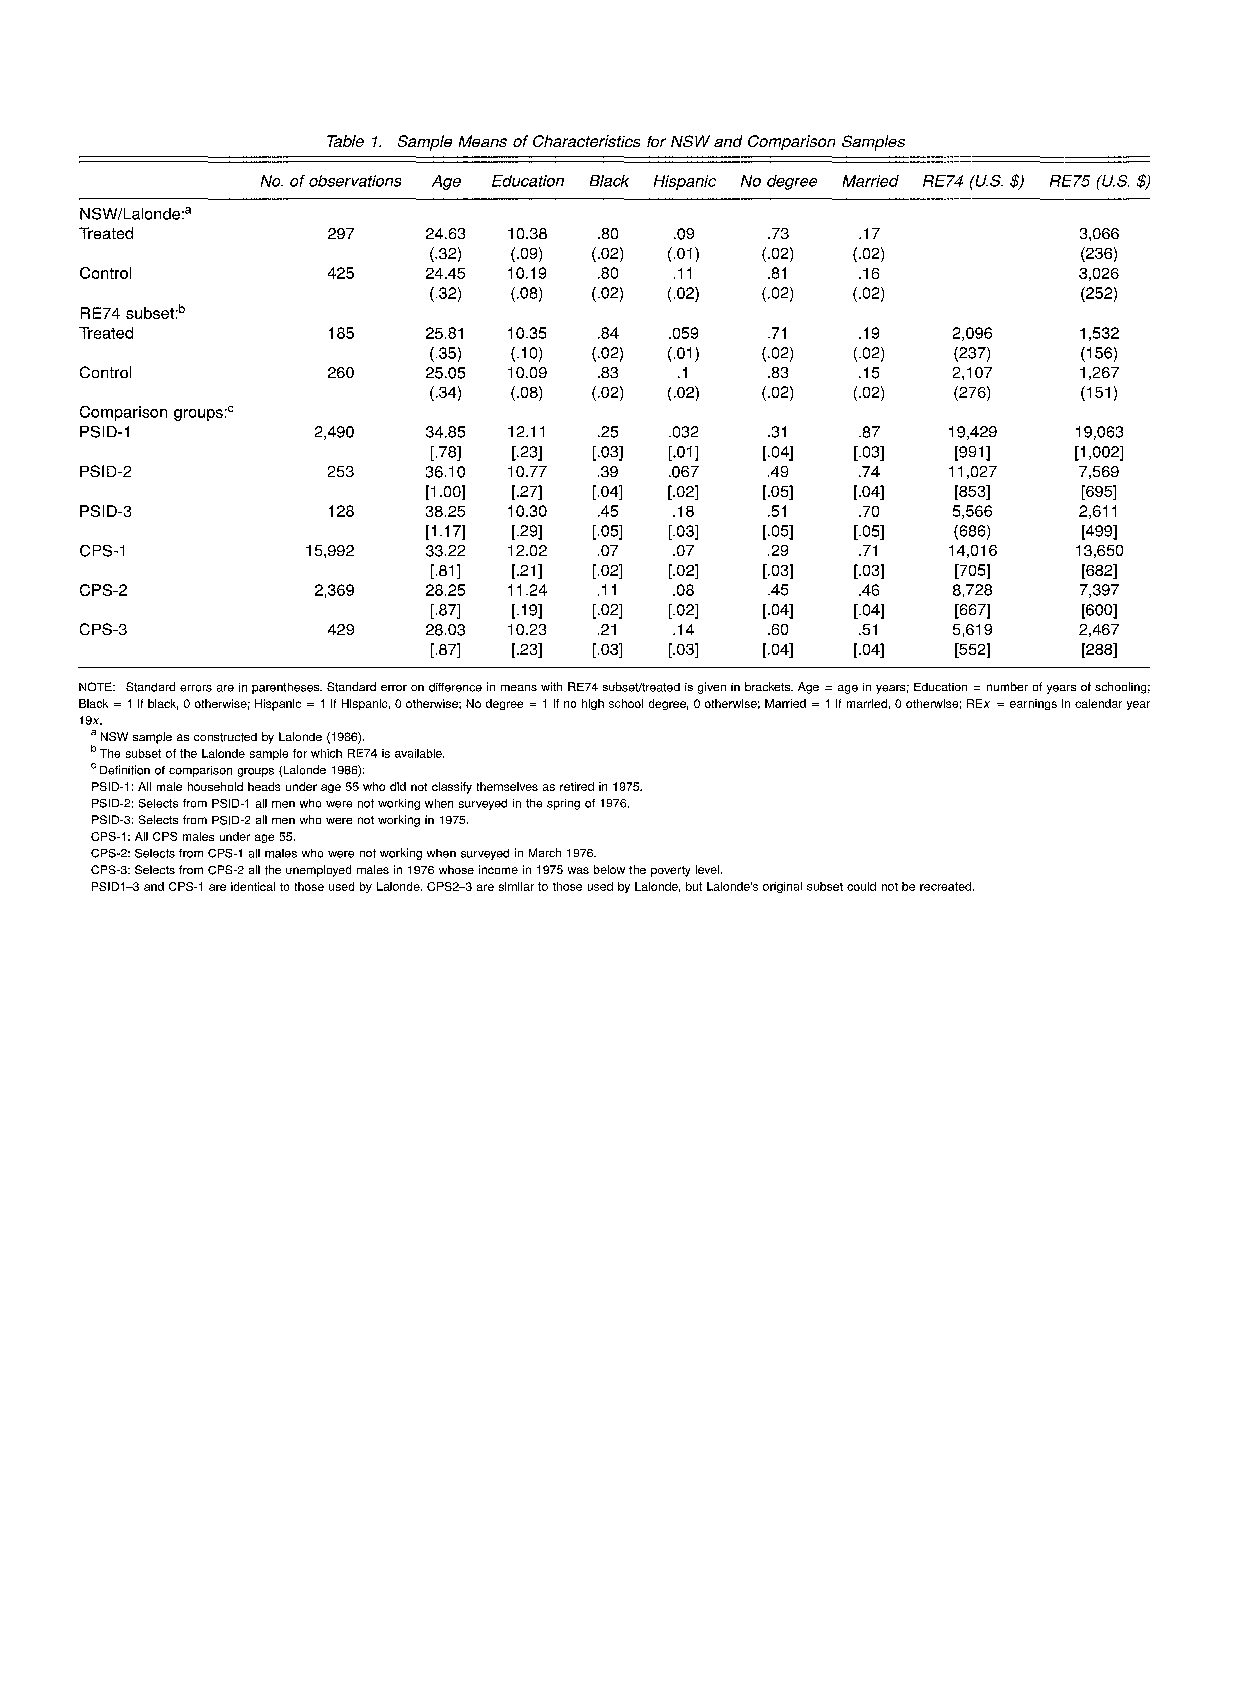
\includegraphics[scale=0.5]{./lecture_includes/dw_1.pdf}
\end{figure}

\end{frame}

\imageframe{./lecture_includes/dw_2.pdf}

\begin{frame}{Proposition 2}
	
	\begin{eqnarray*}
	X \independent D | p(X)
	\end{eqnarray*}
	
	\begin{itemize}
	\item Conditional on the propensity score, the covariates are independent of the treatment, suggesting that the distribution of covariate values should be the same for both treatment and control groups
	\item This can be checked as we have data on all three once we've estimated the propensity score
	\end{itemize}

\end{frame}

\begin{frame}{Trimming the data}
	
	\begin{itemize}
	\item Common terms are ``trimming'' or ``pruning''
	\item Drop units which do not overlap in terms of estimated propensity score
	\item Sometimes as a rule of thumb, just keep units on the \texttt{[0.1,0.9]} interval
	\end{itemize}

\end{frame}


\imageframe{./lecture_includes/dw_3.pdf}
\imageframe{./lecture_includes/dw_4.pdf}
\imageframe{./lecture_includes/dw_5.pdf}
\imageframe{./lecture_includes/dw_6.pdf}





\clearpage
\newpage

\begin{frame}{Subsequent studies}

\begin{itemize}
\item Heckman et al. (1996, 1998) used experimental data from the US National Job Training Partnership Act (JTPA)
\item They conclude that in order for matching estimators to have low bias, it is important that the data include a rich set of variables related to program participation and labor market outcomes, that the nonexperimental comparison group be drawn from the same local labor markets as the participants and the dependent variable (typically earnings) be measured in the same way for participants and nonparticipants
\item All three of these conditions fail to hold in DW (1999, 2002) according to Smith and Todd (2005)
\end{itemize}

\end{frame}


\begin{frame}{Smith and Todd}

\begin{itemize}
\item Difference-in-differences with propensity scores tended to work well in Smith and Todd (2005)
\item But hard to make this a rule, because it's hard to know ex ante if we've specified the propensity score correctly (i.e., have CIA)
\item It is vital you know you're data, if you're going to use these methods, which means understanding at a deep level the way in which selection (i.e., treatment assignment) works in your data
\end{itemize}

\end{frame}


\subsection{Coarsened exact matching}



\begin{frame}{Coarsened exact matching}
	
\begin{itemize}
\item There are two kinds of matching as we've said
	\begin{enumerate}
	\item \emph{Exact matching} matches a treated unit to all of the control units with the same covariate value. Sometimes this is impossible (e.g., continuous covariate). 
	\item \emph{Approximate matching} specifies a metric to find control units that are close to the treated unit. Requires a distance metric, such as Euclidean, Mahalanobis, or the propensity score.  All of which can be implemented in Stata's \texttt{teffects}.
	\end{enumerate}
\item 	Iacus, King and Porro (2011) propose another version of matching they call coarsened exact matching (CEM). Some big picture ideas
\end{itemize}
\end{frame}

\begin{frame}{Checking imbalance}

\begin{itemize}
\item Iacus, King and Porro (2008) say that in practice approximate matching requires setting the matching solution beforehand, then checking for imbalance after.  
\item Start over, repeat, until the user is exhausted by checking for imbalance.
\end{itemize}

\end{frame}

\begin{frame}{CEM Algorithm}
	
\begin{enumerate}
\item Begin with covariates $X$. Make a copy called $X*$
\item Coarsen $X*$ according to user-defined cutpoints or CEM's automatic binning algorithm
	\begin{itemize}
	\item Schooling $\rightarrow$ less than high school, high school, some college, college, post college
	\end{itemize}
\item Create one stratum per unique observation of $X*$ and place each observation in a stratum
\item Assign these strata to the original data, $X$, and drop any observation whose stratum doesn't contain at least one treated and control unit
\end{enumerate}

You then add weights for stratum size and analyze without matching.

\end{frame}

\begin{frame}{Tradeoffs}
	
	\begin{itemize}
	\item Larger bins mean more coarsening.  This results in fewer strata.  
	\item Fewer strata result in more diverse observations within the same strata and thus higher imbalance
	\item CEM prunes both treatment and control group units, which changes the parameter of interest.  Be transparent about this as you're not estimating the ATE or the ATT when you start pruning
	\end{itemize}
	
\end{frame}

\begin{frame}{Benefits}
	
	\begin{itemize}
	\item The key benefit of CEM is that it is in a class of matching methods called \emph{monotonic imbalance bounding}
	\item MIB methods bound the maximum imbalance in some feature of the empirical distributions by an ex ante decision by the user
	\item In CEM, this ex ante choice is the coarsening decision
	\item By choosing the coarsening beforehand, users can control the amount of imbalance in the matching solution
	\item It's also wicked fast.
	\end{itemize}
\end{frame}


\begin{frame}{Imbalance}
	
	\begin{itemize}
	\item There are several ways of measuring imbalance, but here we focus on the $\mathcal{L}_1(f,g)$ measure which is$$\mathcal{L}_1(f,g) = \frac{1}{2} \sum_{l_1 \dots l_k} | f_{l_1 \dots l_k} - g_{l_1 \dots l_k} |$$where the $f$ and $g$ record the relative frequencies for the treatment and control group units.
	\item Perfect global imbalance is indicated by $\mathcal{L}_1=0$.  Larger values indicate larger imbalance between the groups, with a maximum of $\mathcal{L}_1=1$. 
	\end{itemize}
\end{frame}

\begin{frame}{Stata}
	
	\begin{itemize}
	\item Download $\texttt{cem}$ from Stata:  \texttt{ssc install cem, replace}
	\item You will automatically compute the global imbalance measure, as well as several unidimensional measures of imbalance, when using $\texttt{cem}$
	\item I got a $\mathcal{L}_1=0.55$.  What does it mean?
		\begin{itemize}
		\item By itself, it's meaningless.  It's a reference point between matching solutions.
		\item Once we have a matching solution, we will compare its $\mathcal{L}_1$ to 0.55 and gauge the increase in balance due to the matching solution from that difference.
		\item Thus $\mathcal{L}_1$ works for imbalance as $R^2$ works for model fit: the absolute values mean less than comparisons between matching solutions.
		\end{itemize}
	\end{itemize}
	
\end{frame}

\begin{frame}{More Stata}
	
	\begin{itemize}
	\item Because $\texttt{cem}$ bounds the imbalance ex ante, the most important information in the Stata output is the number of observations matched.
	\item You can also choose the coarsening as opposed to relying on the algorithm's automated binning.  
	\item Once you have estimated the strata, you regress the outcome onto the treatment and then weight the regression by $\texttt{cem_weights}$.  For instance, $$\texttt{regress re78 treat [iweight=cem\_weight]}$$
	\item For more on this, see Blackwell, et al. Stata journal article from 2009.  
	\end{itemize}
\end{frame}







\end{document}
